\documentclass[twoside]{book}

% Packages required by doxygen
\usepackage{fixltx2e}
\usepackage{calc}
\usepackage{doxygen}
\usepackage[export]{adjustbox} % also loads graphicx
\usepackage{graphicx}
\usepackage[utf8]{inputenc}
\usepackage{makeidx}
\usepackage{multicol}
\usepackage{multirow}
\PassOptionsToPackage{warn}{textcomp}
\usepackage{textcomp}
\usepackage[nointegrals]{wasysym}
\usepackage[table]{xcolor}

% Font selection
\usepackage[T1]{fontenc}
\usepackage[scaled=.90]{helvet}
\usepackage{courier}
\usepackage{amssymb}
\usepackage{sectsty}
\renewcommand{\familydefault}{\sfdefault}
\allsectionsfont{%
  \fontseries{bc}\selectfont%
  \color{darkgray}%
}
\renewcommand{\DoxyLabelFont}{%
  \fontseries{bc}\selectfont%
  \color{darkgray}%
}
\newcommand{\+}{\discretionary{\mbox{\scriptsize$\hookleftarrow$}}{}{}}

% Page & text layout
\usepackage{geometry}
\geometry{%
  a4paper,%
  top=2.5cm,%
  bottom=2.5cm,%
  left=2.5cm,%
  right=2.5cm%
}
\tolerance=750
\hfuzz=15pt
\hbadness=750
\setlength{\emergencystretch}{15pt}
\setlength{\parindent}{0cm}
\setlength{\parskip}{3ex plus 2ex minus 2ex}
\makeatletter
\renewcommand{\paragraph}{%
  \@startsection{paragraph}{4}{0ex}{-1.0ex}{1.0ex}{%
    \normalfont\normalsize\bfseries\SS@parafont%
  }%
}
\renewcommand{\subparagraph}{%
  \@startsection{subparagraph}{5}{0ex}{-1.0ex}{1.0ex}{%
    \normalfont\normalsize\bfseries\SS@subparafont%
  }%
}
\makeatother

% Headers & footers
\usepackage{fancyhdr}
\pagestyle{fancyplain}
\fancyhead[LE]{\fancyplain{}{\bfseries\thepage}}
\fancyhead[CE]{\fancyplain{}{}}
\fancyhead[RE]{\fancyplain{}{\bfseries\leftmark}}
\fancyhead[LO]{\fancyplain{}{\bfseries\rightmark}}
\fancyhead[CO]{\fancyplain{}{}}
\fancyhead[RO]{\fancyplain{}{\bfseries\thepage}}
\fancyfoot[LE]{\fancyplain{}{}}
\fancyfoot[CE]{\fancyplain{}{}}
\fancyfoot[RE]{\fancyplain{}{\bfseries\scriptsize Generated by Doxygen }}
\fancyfoot[LO]{\fancyplain{}{\bfseries\scriptsize Generated by Doxygen }}
\fancyfoot[CO]{\fancyplain{}{}}
\fancyfoot[RO]{\fancyplain{}{}}
\renewcommand{\footrulewidth}{0.4pt}
\renewcommand{\chaptermark}[1]{%
  \markboth{#1}{}%
}
\renewcommand{\sectionmark}[1]{%
  \markright{\thesection\ #1}%
}

% Indices & bibliography
\usepackage{natbib}
\usepackage[titles]{tocloft}
\setcounter{tocdepth}{3}
\setcounter{secnumdepth}{5}
\makeindex

% Hyperlinks (required, but should be loaded last)
\usepackage{ifpdf}
\ifpdf
  \usepackage[pdftex,pagebackref=true]{hyperref}
\else
  \usepackage[ps2pdf,pagebackref=true]{hyperref}
\fi
\hypersetup{%
  colorlinks=true,%
  linkcolor=blue,%
  citecolor=blue,%
  unicode%
}

% Custom commands
\newcommand{\clearemptydoublepage}{%
  \newpage{\pagestyle{empty}\cleardoublepage}%
}

\usepackage{caption}
\captionsetup{labelsep=space,justification=centering,font={bf},singlelinecheck=off,skip=4pt,position=top}

%===== C O N T E N T S =====

\begin{document}

% Titlepage & ToC
\hypersetup{pageanchor=false,
             bookmarksnumbered=true,
             pdfencoding=unicode
            }
\pagenumbering{roman}
\begin{titlepage}
\vspace*{7cm}
\begin{center}%
{\Large My Project }\\
\vspace*{1cm}
{\large Generated by Doxygen 1.8.11}\\
\end{center}
\end{titlepage}
\clearemptydoublepage
\tableofcontents
\clearemptydoublepage
\pagenumbering{arabic}
\hypersetup{pageanchor=true}

%--- Begin generated contents ---
\chapter{Graphs-\/in-\/C}
\label{md_README}
\hypertarget{md_README}{}
This is a simple graph-\/library written in pure C. The example shows how to find an eulerian path in a graph, loaded from a text file. 
\chapter{Data Structure Index}
\section{Data Structures}
Here are the data structures with brief descriptions\+:\begin{DoxyCompactList}
\item\contentsline{section}{\hyperlink{structComparator}{Comparator} \\*An object to compare data }{\pageref{structComparator}}{}
\item\contentsline{section}{\hyperlink{structDList}{D\+List} \\*The data structure of a generic doubly linked list }{\pageref{structDList}}{}
\item\contentsline{section}{\hyperlink{structDListIterator}{D\+List\+Iterator} \\*A simple bidirectional iterator }{\pageref{structDListIterator}}{}
\item\contentsline{section}{\hyperlink{structDListNode}{D\+List\+Node} \\*The atomic data structure of a generic doubly linked list. (\hyperlink{structDList}{D\+List}) }{\pageref{structDListNode}}{}
\item\contentsline{section}{\hyperlink{structEdge}{Edge} }{\pageref{structEdge}}{}
\item\contentsline{section}{\hyperlink{structEulerianCycleResult}{Eulerian\+Cycle\+Result} }{\pageref{structEulerianCycleResult}}{}
\item\contentsline{section}{\hyperlink{structGraph}{Graph} }{\pageref{structGraph}}{}
\item\contentsline{section}{\hyperlink{structGraphInformation}{Graph\+Information} }{\pageref{structGraphInformation}}{}
\item\contentsline{section}{\hyperlink{structPath}{Path} \\*This is just a container for a list of path elements which simply represent the vertices }{\pageref{structPath}}{}
\item\contentsline{section}{\hyperlink{structPathElement}{Path\+Element} }{\pageref{structPathElement}}{}
\item\contentsline{section}{\hyperlink{structVertex}{Vertex} \\*A vertex in a graph is just a container of a doubly linked list of edges }{\pageref{structVertex}}{}
\end{DoxyCompactList}

\chapter{File Index}
\section{File List}
Here is a list of all documented files with brief descriptions\+:\begin{DoxyCompactList}
\item\contentsline{section}{\hyperlink{basic_8h}{basic.\+h} \\*Just some arbitrary definitions for the library }{\pageref{basic_8h}}{}
\item\contentsline{section}{\hyperlink{comparator_8h}{comparator.\+h} \\*An object to compare data. As an example, it can be used to search data in a list }{\pageref{comparator_8h}}{}
\item\contentsline{section}{\hyperlink{dlist_8h}{dlist.\+h} \\*A generic doubly linked list }{\pageref{dlist_8h}}{}
\item\contentsline{section}{\hyperlink{dlistiterator_8h}{dlistiterator.\+h} \\*A bidirectional iterator for a doubly linked list }{\pageref{dlistiterator_8h}}{}
\item\contentsline{section}{\hyperlink{dlistnode_8h}{dlistnode.\+h} \\*A node in a generic doubly linked list }{\pageref{dlistnode_8h}}{}
\item\contentsline{section}{\hyperlink{edge_8h}{edge.\+h} \\*The edge between vertices in a graph }{\pageref{edge_8h}}{}
\item\contentsline{section}{\hyperlink{graph_8h}{graph.\+h} \\*A graph containing vertices which are connected through edges }{\pageref{graph_8h}}{}
\item\contentsline{section}{\hyperlink{path_8h}{path.\+h} \\*A path of vertices of a graph }{\pageref{path_8h}}{}
\item\contentsline{section}{\hyperlink{pathelement_8h}{pathelement.\+h} \\*An element of a path of a graph }{\pageref{pathelement_8h}}{}
\item\contentsline{section}{\hyperlink{vertex_8h}{vertex.\+h} \\*A vertex in a graph }{\pageref{vertex_8h}}{}
\end{DoxyCompactList}

\chapter{Data Structure Documentation}
\hypertarget{structComparator}{}\section{Comparator Struct Reference}
\label{structComparator}\index{Comparator@{Comparator}}


An object to compare data.  




{\ttfamily \#include $<$comparator.\+h$>$}

\subsection*{Data Fields}
\begin{DoxyCompactItemize}
\item 
\hyperlink{basic_8h_a5f051eaa796886555205c751e6d530f4}{Data} \hyperlink{structComparator_a6d1641e7a7be309c8aeb308f4b9032af}{data}
\item 
\hyperlink{comparator_8h_a7031dbbb6ddea05773826b8d54940494}{Compare\+Function} \hyperlink{structComparator_aa308e51b1d9b8ad152c7f36c3001dc7d}{compare\+Function}
\end{DoxyCompactItemize}


\subsection{Detailed Description}
An object to compare data. 

\subsection{Field Documentation}
\index{Comparator@{Comparator}!compare\+Function@{compare\+Function}}
\index{compare\+Function@{compare\+Function}!Comparator@{Comparator}}
\subsubsection[{\texorpdfstring{compare\+Function}{compareFunction}}]{\setlength{\rightskip}{0pt plus 5cm}{\bf Compare\+Function} Comparator\+::compare\+Function}\hypertarget{structComparator_aa308e51b1d9b8ad152c7f36c3001dc7d}{}\label{structComparator_aa308e51b1d9b8ad152c7f36c3001dc7d}
The compare function to evaluate if the stored data and some input data is matching the implemented compare criteria. \index{Comparator@{Comparator}!data@{data}}
\index{data@{data}!Comparator@{Comparator}}
\subsubsection[{\texorpdfstring{data}{data}}]{\setlength{\rightskip}{0pt plus 5cm}{\bf Data} Comparator\+::data}\hypertarget{structComparator_a6d1641e7a7be309c8aeb308f4b9032af}{}\label{structComparator_a6d1641e7a7be309c8aeb308f4b9032af}
Data stored, to compare with other data. 

The documentation for this struct was generated from the following file\+:\begin{DoxyCompactItemize}
\item 
\hyperlink{comparator_8h}{comparator.\+h}\end{DoxyCompactItemize}

\hypertarget{structDList}{}\section{D\+List Struct Reference}
\label{structDList}\index{D\+List@{D\+List}}


The data structure of a generic doubly linked list.  




{\ttfamily \#include $<$dlist.\+h$>$}



Collaboration diagram for D\+List\+:\nopagebreak
\begin{figure}[H]
\begin{center}
\leavevmode
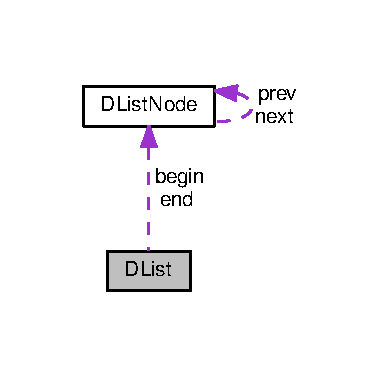
\includegraphics[width=183pt]{structDList__coll__graph}
\end{center}
\end{figure}
\subsection*{Data Fields}
\begin{DoxyCompactItemize}
\item 
int \hyperlink{structDList_aac5e5498f12e33cdcf9212802b92ded4}{data\+Size}
\item 
int \hyperlink{structDList_a85d2c4c3a5abba8fb8c903571ae72369}{list\+Size}
\item 
\hyperlink{structDListNode}{D\+List\+Node} $\ast$ \hyperlink{structDList_a9f124f116c54de297ae53584cb3a13f6}{begin}
\item 
\hyperlink{structDListNode}{D\+List\+Node} $\ast$ \hyperlink{structDList_ae11ba36cd0e3bdeac4c7189910993864}{end}
\item 
\hyperlink{dlist_8h_a2206207e78cb6335a8f41ad6cf76b55c}{Destroy\+Function} \hyperlink{structDList_a039e1b8cd416fceafdb407c1bc51ae4c}{destroy\+Function}
\end{DoxyCompactItemize}


\subsection{Detailed Description}
The data structure of a generic doubly linked list. 

The \hyperlink{structDList}{D\+List} is made up of at least two nodes\+: The begin and the end node of the list. These nodes will be created when the list is created and will never be removed from the list until the list is destroyed. Thus, the begin and end nodes will have a N\+U\+LL pointer to their data. They\textquotesingle{}re empty objects. Having discrete nodes for the begin and end of the list will result in fewer checks compared to lists without them.

Some defintions\+: 
\begin{DoxyCode}
An \textcolor{stringliteral}{'empty'} list:
    A list which has no nodes other than the discrete \hyperlink{structDList_a9f124f116c54de297ae53584cb3a13f6}{begin} and \hyperlink{structDList_ae11ba36cd0e3bdeac4c7189910993864}{end} nodes.

The \textcolor{stringliteral}{'first'} node of the list:
    IF the list is not empty    -> The next node of the discrete \hyperlink{structDList_a9f124f116c54de297ae53584cb3a13f6}{begin} node
    ELSE                        -> A \textcolor{stringliteral}{'first'} node does not exist / is undefined.

The \textcolor{stringliteral}{'last'} node of the list:
    IF the list is not empty    -> The previous node of the discrete \hyperlink{structDList_ae11ba36cd0e3bdeac4c7189910993864}{end} node
    ELSE                        -> A \textcolor{stringliteral}{'last'} node does not exist / is undefined.
\end{DoxyCode}
 

\subsection{Field Documentation}
\index{D\+List@{D\+List}!begin@{begin}}
\index{begin@{begin}!D\+List@{D\+List}}
\subsubsection[{\texorpdfstring{begin}{begin}}]{\setlength{\rightskip}{0pt plus 5cm}{\bf D\+List\+Node}$\ast$ D\+List\+::begin}\hypertarget{structDList_a9f124f116c54de297ae53584cb3a13f6}{}\label{structDList_a9f124f116c54de297ae53584cb3a13f6}
The discrete begin node of the list. \index{D\+List@{D\+List}!data\+Size@{data\+Size}}
\index{data\+Size@{data\+Size}!D\+List@{D\+List}}
\subsubsection[{\texorpdfstring{data\+Size}{dataSize}}]{\setlength{\rightskip}{0pt plus 5cm}int D\+List\+::data\+Size}\hypertarget{structDList_aac5e5498f12e33cdcf9212802b92ded4}{}\label{structDList_aac5e5498f12e33cdcf9212802b92ded4}
The size of the data stored in each node. \index{D\+List@{D\+List}!destroy\+Function@{destroy\+Function}}
\index{destroy\+Function@{destroy\+Function}!D\+List@{D\+List}}
\subsubsection[{\texorpdfstring{destroy\+Function}{destroyFunction}}]{\setlength{\rightskip}{0pt plus 5cm}{\bf Destroy\+Function} D\+List\+::destroy\+Function}\hypertarget{structDList_a039e1b8cd416fceafdb407c1bc51ae4c}{}\label{structDList_a039e1b8cd416fceafdb407c1bc51ae4c}
A function which destroys the data of a node. \index{D\+List@{D\+List}!end@{end}}
\index{end@{end}!D\+List@{D\+List}}
\subsubsection[{\texorpdfstring{end}{end}}]{\setlength{\rightskip}{0pt plus 5cm}{\bf D\+List\+Node}$\ast$ D\+List\+::end}\hypertarget{structDList_ae11ba36cd0e3bdeac4c7189910993864}{}\label{structDList_ae11ba36cd0e3bdeac4c7189910993864}
The discrete end node of the list. \index{D\+List@{D\+List}!list\+Size@{list\+Size}}
\index{list\+Size@{list\+Size}!D\+List@{D\+List}}
\subsubsection[{\texorpdfstring{list\+Size}{listSize}}]{\setlength{\rightskip}{0pt plus 5cm}int D\+List\+::list\+Size}\hypertarget{structDList_a85d2c4c3a5abba8fb8c903571ae72369}{}\label{structDList_a85d2c4c3a5abba8fb8c903571ae72369}
The number of nodes in the list excluding the begin and end nodes. 

The documentation for this struct was generated from the following file\+:\begin{DoxyCompactItemize}
\item 
\hyperlink{dlist_8h}{dlist.\+h}\end{DoxyCompactItemize}

\hypertarget{structDListIterator}{}\section{D\+List\+Iterator Struct Reference}
\label{structDListIterator}\index{D\+List\+Iterator@{D\+List\+Iterator}}


A simple bidirectional iterator.  




{\ttfamily \#include $<$dlistiterator.\+h$>$}



Collaboration diagram for D\+List\+Iterator\+:\nopagebreak
\begin{figure}[H]
\begin{center}
\leavevmode
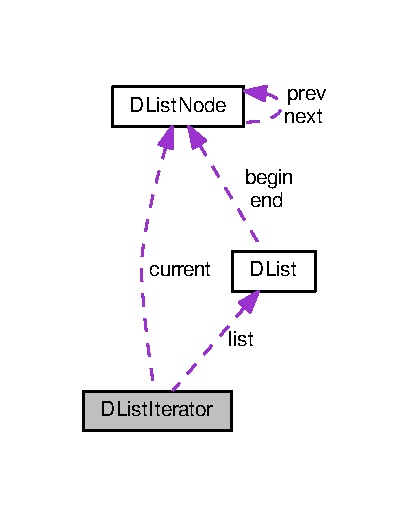
\includegraphics[width=197pt]{structDListIterator__coll__graph}
\end{center}
\end{figure}
\subsection*{Data Fields}
\begin{DoxyCompactItemize}
\item 
\hyperlink{structDList}{D\+List} $\ast$ \hyperlink{structDListIterator_ad948282c06cc2a1c796699443404c73f}{list}
\item 
\hyperlink{structDListNode}{D\+List\+Node} $\ast$ \hyperlink{structDListIterator_a5f347829fbf97fb211160150628db997}{current}
\end{DoxyCompactItemize}


\subsection{Detailed Description}
A simple bidirectional iterator. 

\subsection{Field Documentation}
\index{D\+List\+Iterator@{D\+List\+Iterator}!current@{current}}
\index{current@{current}!D\+List\+Iterator@{D\+List\+Iterator}}
\subsubsection[{\texorpdfstring{current}{current}}]{\setlength{\rightskip}{0pt plus 5cm}{\bf D\+List\+Node}$\ast$ D\+List\+Iterator\+::current}\hypertarget{structDListIterator_a5f347829fbf97fb211160150628db997}{}\label{structDListIterator_a5f347829fbf97fb211160150628db997}
The node to interact with in the list. \index{D\+List\+Iterator@{D\+List\+Iterator}!list@{list}}
\index{list@{list}!D\+List\+Iterator@{D\+List\+Iterator}}
\subsubsection[{\texorpdfstring{list}{list}}]{\setlength{\rightskip}{0pt plus 5cm}{\bf D\+List}$\ast$ D\+List\+Iterator\+::list}\hypertarget{structDListIterator_ad948282c06cc2a1c796699443404c73f}{}\label{structDListIterator_ad948282c06cc2a1c796699443404c73f}
The list which the iterator iterates over. 

The documentation for this struct was generated from the following file\+:\begin{DoxyCompactItemize}
\item 
\hyperlink{dlistiterator_8h}{dlistiterator.\+h}\end{DoxyCompactItemize}

\hypertarget{structDListNode}{}\section{D\+List\+Node Struct Reference}
\label{structDListNode}\index{D\+List\+Node@{D\+List\+Node}}


The atomic data structure of a generic doubly linked list. (\hyperlink{structDList}{D\+List})  




{\ttfamily \#include $<$dlistnode.\+h$>$}



Collaboration diagram for D\+List\+Node\+:\nopagebreak
\begin{figure}[H]
\begin{center}
\leavevmode
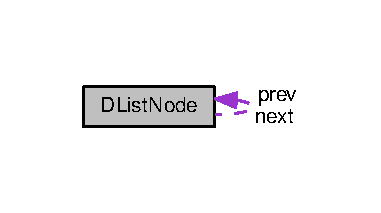
\includegraphics[width=183pt]{structDListNode__coll__graph}
\end{center}
\end{figure}
\subsection*{Data Fields}
\begin{DoxyCompactItemize}
\item 
\hyperlink{basic_8h_a5f051eaa796886555205c751e6d530f4}{Data} \hyperlink{structDListNode_aae5a2c880ddfb133d04d97910f356e6b}{data}
\item 
\hyperlink{structDListNode}{D\+List\+Node} $\ast$ \hyperlink{structDListNode_af52bb1206b2228c7e47eb5ecd5dbb38d}{prev}
\item 
\hyperlink{structDListNode}{D\+List\+Node} $\ast$ \hyperlink{structDListNode_af9d7a8fe9c70f6836aba009163392fcc}{next}
\end{DoxyCompactItemize}


\subsection{Detailed Description}
The atomic data structure of a generic doubly linked list. (\hyperlink{structDList}{D\+List}) 

\subsection{Field Documentation}
\index{D\+List\+Node@{D\+List\+Node}!data@{data}}
\index{data@{data}!D\+List\+Node@{D\+List\+Node}}
\subsubsection[{\texorpdfstring{data}{data}}]{\setlength{\rightskip}{0pt plus 5cm}{\bf Data} D\+List\+Node\+::data}\hypertarget{structDListNode_aae5a2c880ddfb133d04d97910f356e6b}{}\label{structDListNode_aae5a2c880ddfb133d04d97910f356e6b}
The generic data. \index{D\+List\+Node@{D\+List\+Node}!next@{next}}
\index{next@{next}!D\+List\+Node@{D\+List\+Node}}
\subsubsection[{\texorpdfstring{next}{next}}]{\setlength{\rightskip}{0pt plus 5cm}{\bf D\+List\+Node}$\ast$ D\+List\+Node\+::next}\hypertarget{structDListNode_af9d7a8fe9c70f6836aba009163392fcc}{}\label{structDListNode_af9d7a8fe9c70f6836aba009163392fcc}
The next node. \index{D\+List\+Node@{D\+List\+Node}!prev@{prev}}
\index{prev@{prev}!D\+List\+Node@{D\+List\+Node}}
\subsubsection[{\texorpdfstring{prev}{prev}}]{\setlength{\rightskip}{0pt plus 5cm}{\bf D\+List\+Node}$\ast$ D\+List\+Node\+::prev}\hypertarget{structDListNode_af52bb1206b2228c7e47eb5ecd5dbb38d}{}\label{structDListNode_af52bb1206b2228c7e47eb5ecd5dbb38d}
The previous node. 

The documentation for this struct was generated from the following file\+:\begin{DoxyCompactItemize}
\item 
\hyperlink{dlistnode_8h}{dlistnode.\+h}\end{DoxyCompactItemize}

\hypertarget{structEdge}{}\section{Edge Struct Reference}
\label{structEdge}\index{Edge@{Edge}}


Collaboration diagram for Edge\+:\nopagebreak
\begin{figure}[H]
\begin{center}
\leavevmode
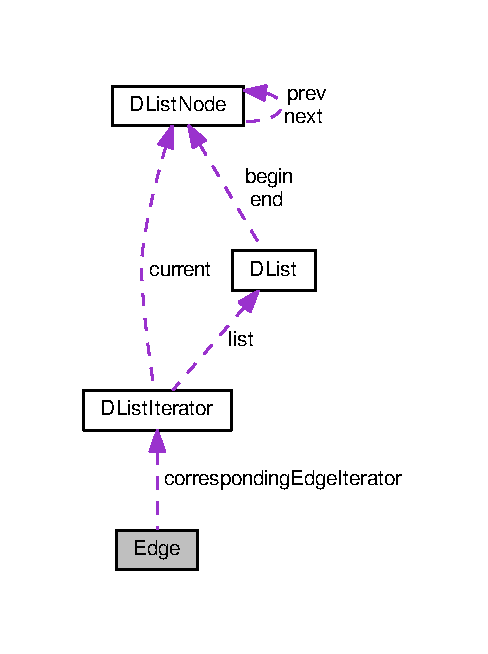
\includegraphics[width=234pt]{structEdge__coll__graph}
\end{center}
\end{figure}
\subsection*{Data Fields}
\begin{DoxyCompactItemize}
\item 
int \hyperlink{structEdge_affa54ce2dd876532f6b87fc049f5bd7d}{to\+Vertex\+Num}
\item 
\hyperlink{structDListIterator}{D\+List\+Iterator} $\ast$ \hyperlink{structEdge_a3cf54ba60e278bb26d3b39756f806ea1}{corresponding\+Edge\+Iterator}
\end{DoxyCompactItemize}


\subsection{Field Documentation}
\index{Edge@{Edge}!corresponding\+Edge\+Iterator@{corresponding\+Edge\+Iterator}}
\index{corresponding\+Edge\+Iterator@{corresponding\+Edge\+Iterator}!Edge@{Edge}}
\subsubsection[{\texorpdfstring{corresponding\+Edge\+Iterator}{correspondingEdgeIterator}}]{\setlength{\rightskip}{0pt plus 5cm}{\bf D\+List\+Iterator}$\ast$ Edge\+::corresponding\+Edge\+Iterator}\hypertarget{structEdge_a3cf54ba60e278bb26d3b39756f806ea1}{}\label{structEdge_a3cf54ba60e278bb26d3b39756f806ea1}
An iterator to \index{Edge@{Edge}!to\+Vertex\+Num@{to\+Vertex\+Num}}
\index{to\+Vertex\+Num@{to\+Vertex\+Num}!Edge@{Edge}}
\subsubsection[{\texorpdfstring{to\+Vertex\+Num}{toVertexNum}}]{\setlength{\rightskip}{0pt plus 5cm}int Edge\+::to\+Vertex\+Num}\hypertarget{structEdge_affa54ce2dd876532f6b87fc049f5bd7d}{}\label{structEdge_affa54ce2dd876532f6b87fc049f5bd7d}
The vertex number of the vertex this edge goes to. 

The documentation for this struct was generated from the following file\+:\begin{DoxyCompactItemize}
\item 
\hyperlink{edge_8h}{edge.\+h}\end{DoxyCompactItemize}

\hypertarget{structEulerianCycleResult}{}\section{Eulerian\+Cycle\+Result Struct Reference}
\label{structEulerianCycleResult}\index{Eulerian\+Cycle\+Result@{Eulerian\+Cycle\+Result}}


Collaboration diagram for Eulerian\+Cycle\+Result\+:\nopagebreak
\begin{figure}[H]
\begin{center}
\leavevmode
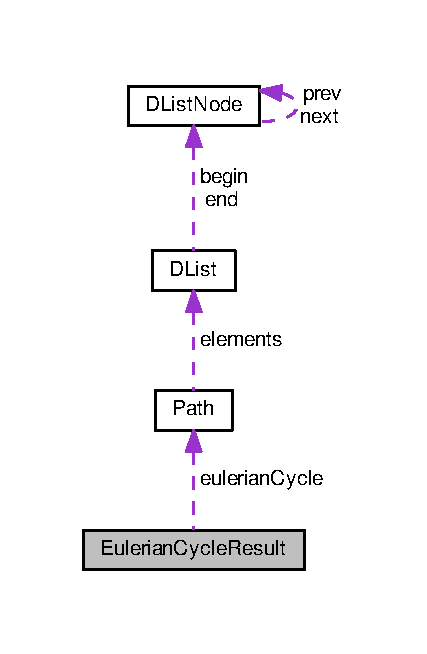
\includegraphics[width=205pt]{structEulerianCycleResult__coll__graph}
\end{center}
\end{figure}
\subsection*{Data Fields}
\begin{DoxyCompactItemize}
\item 
bool {\bfseries exists}\hypertarget{structEulerianCycleResult_a669d96b44b92364e7beee4f0addc8713}{}\label{structEulerianCycleResult_a669d96b44b92364e7beee4f0addc8713}

\item 
\hyperlink{structPath}{Path} $\ast$ {\bfseries eulerian\+Cycle}\hypertarget{structEulerianCycleResult_ac6330c5f78f7c1be7f0666645064d986}{}\label{structEulerianCycleResult_ac6330c5f78f7c1be7f0666645064d986}

\end{DoxyCompactItemize}


The documentation for this struct was generated from the following file\+:\begin{DoxyCompactItemize}
\item 
main.\+c\end{DoxyCompactItemize}

\hypertarget{structGraph}{}\section{Graph Struct Reference}
\label{structGraph}\index{Graph@{Graph}}


Collaboration diagram for Graph\+:\nopagebreak
\begin{figure}[H]
\begin{center}
\leavevmode
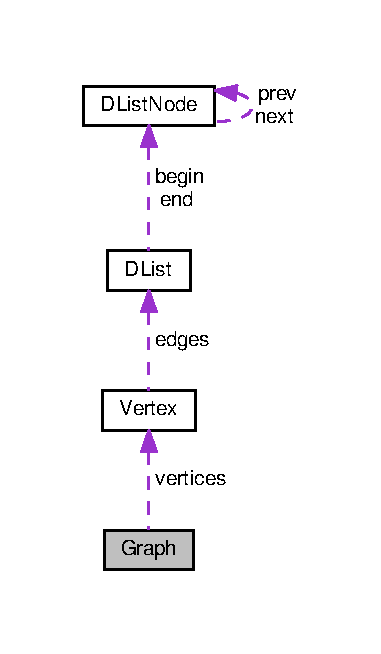
\includegraphics[width=183pt]{structGraph__coll__graph}
\end{center}
\end{figure}
\subsection*{Data Fields}
\begin{DoxyCompactItemize}
\item 
\hyperlink{structVertex}{Vertex} $\ast$$\ast$ {\bfseries vertices}\hypertarget{structGraph_a78b1f05b8d7d75efa2da1688f7ab4e85}{}\label{structGraph_a78b1f05b8d7d75efa2da1688f7ab4e85}

\item 
int {\bfseries vertex\+Count}\hypertarget{structGraph_aa61a470b538b8c5836ae3f3e6a4dc438}{}\label{structGraph_aa61a470b538b8c5836ae3f3e6a4dc438}

\end{DoxyCompactItemize}


The documentation for this struct was generated from the following file\+:\begin{DoxyCompactItemize}
\item 
graph.\+h\end{DoxyCompactItemize}

\hypertarget{structGraphInformation}{}\section{Graph\+Information Struct Reference}
\label{structGraphInformation}\index{Graph\+Information@{Graph\+Information}}
\subsection*{Data Fields}
\begin{DoxyCompactItemize}
\item 
Graph\+Type {\bfseries graph\+Type}\hypertarget{structGraphInformation_a525b30e8a6065f7a4f586c3ec07312e6}{}\label{structGraphInformation_a525b30e8a6065f7a4f586c3ec07312e6}

\item 
int {\bfseries start\+Or\+End\+Vertex\+Num1}\hypertarget{structGraphInformation_a724f3a89e48c6fc29ba45e0df0b319e4}{}\label{structGraphInformation_a724f3a89e48c6fc29ba45e0df0b319e4}

\item 
int {\bfseries start\+Or\+End\+Vertex\+Num2}\hypertarget{structGraphInformation_a0833742e1c1241684231ad082661e514}{}\label{structGraphInformation_a0833742e1c1241684231ad082661e514}

\item 
int {\bfseries vertex\+With\+Max\+Degree}\hypertarget{structGraphInformation_aa5040463d22d2a57806c7276767f8371}{}\label{structGraphInformation_aa5040463d22d2a57806c7276767f8371}

\end{DoxyCompactItemize}


The documentation for this struct was generated from the following file\+:\begin{DoxyCompactItemize}
\item 
main.\+c\end{DoxyCompactItemize}

\hypertarget{structPath}{}\section{Path Struct Reference}
\label{structPath}\index{Path@{Path}}


Collaboration diagram for Path\+:\nopagebreak
\begin{figure}[H]
\begin{center}
\leavevmode
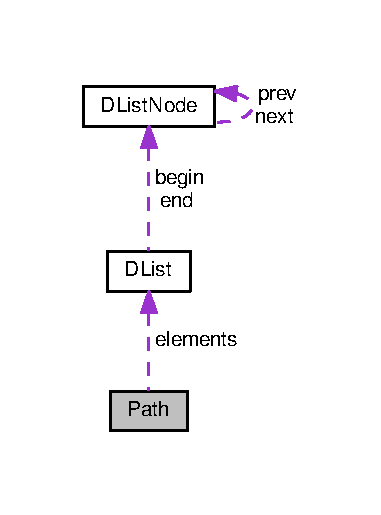
\includegraphics[width=183pt]{structPath__coll__graph}
\end{center}
\end{figure}
\subsection*{Data Fields}
\begin{DoxyCompactItemize}
\item 
\hyperlink{structDList}{D\+List} $\ast$ {\bfseries elements}\hypertarget{structPath_a9767e852a01fe98f15198cc23538aad0}{}\label{structPath_a9767e852a01fe98f15198cc23538aad0}

\end{DoxyCompactItemize}


The documentation for this struct was generated from the following file\+:\begin{DoxyCompactItemize}
\item 
path.\+h\end{DoxyCompactItemize}

\hypertarget{structPathElement}{}\section{Path\+Element Struct Reference}
\label{structPathElement}\index{Path\+Element@{Path\+Element}}


{\ttfamily \#include $<$pathelement.\+h$>$}

\subsection*{Data Fields}
\begin{DoxyCompactItemize}
\item 
int \hyperlink{structPathElement_a1f2bbaf04337046497c6ac63d96062a7}{vertex\+Num}
\end{DoxyCompactItemize}


\subsection{Detailed Description}
A path element contains simply a vertex number. 

\subsection{Field Documentation}
\index{Path\+Element@{Path\+Element}!vertex\+Num@{vertex\+Num}}
\index{vertex\+Num@{vertex\+Num}!Path\+Element@{Path\+Element}}
\subsubsection[{\texorpdfstring{vertex\+Num}{vertexNum}}]{\setlength{\rightskip}{0pt plus 5cm}int Path\+Element\+::vertex\+Num}\hypertarget{structPathElement_a1f2bbaf04337046497c6ac63d96062a7}{}\label{structPathElement_a1f2bbaf04337046497c6ac63d96062a7}
The vertex number this element represents. 

The documentation for this struct was generated from the following file\+:\begin{DoxyCompactItemize}
\item 
\hyperlink{pathelement_8h}{pathelement.\+h}\end{DoxyCompactItemize}

\hypertarget{structVertex}{}\section{Vertex Struct Reference}
\label{structVertex}\index{Vertex@{Vertex}}


A vertex in a graph is just a container of a doubly linked list of edges.  




{\ttfamily \#include $<$vertex.\+h$>$}



Collaboration diagram for Vertex\+:\nopagebreak
\begin{figure}[H]
\begin{center}
\leavevmode
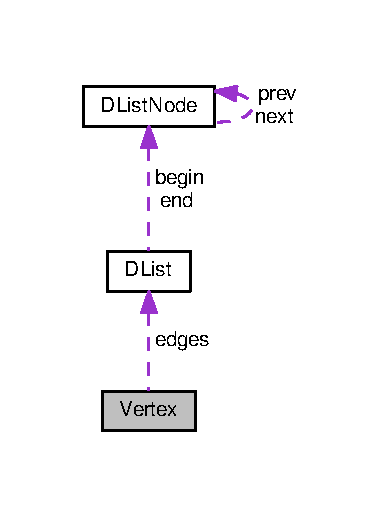
\includegraphics[width=183pt]{structVertex__coll__graph}
\end{center}
\end{figure}
\subsection*{Data Fields}
\begin{DoxyCompactItemize}
\item 
\hyperlink{structDList}{D\+List} $\ast$ \hyperlink{structVertex_a1d47f7cbd5679ba2c22c556b39f994a8}{edges}
\end{DoxyCompactItemize}


\subsection{Detailed Description}
A vertex in a graph is just a container of a doubly linked list of edges. 

\subsection{Field Documentation}
\index{Vertex@{Vertex}!edges@{edges}}
\index{edges@{edges}!Vertex@{Vertex}}
\subsubsection[{\texorpdfstring{edges}{edges}}]{\setlength{\rightskip}{0pt plus 5cm}{\bf D\+List}$\ast$ Vertex\+::edges}\hypertarget{structVertex_a1d47f7cbd5679ba2c22c556b39f994a8}{}\label{structVertex_a1d47f7cbd5679ba2c22c556b39f994a8}
The list of edges. 

The documentation for this struct was generated from the following file\+:\begin{DoxyCompactItemize}
\item 
\hyperlink{vertex_8h}{vertex.\+h}\end{DoxyCompactItemize}

\chapter{File Documentation}
\hypertarget{basic_8h}{}\section{basic.\+h File Reference}
\label{basic_8h}\index{basic.\+h@{basic.\+h}}


Just some arbitrary definitions for the library.  


{\ttfamily \#include \char`\"{}assert.\+h\char`\"{}}\\*
{\ttfamily \#include \char`\"{}stdlib.\+h\char`\"{}}\\*
{\ttfamily \#include \char`\"{}stdio.\+h\char`\"{}}\\*
Include dependency graph for basic.\+h\+:
\nopagebreak
\begin{figure}[H]
\begin{center}
\leavevmode
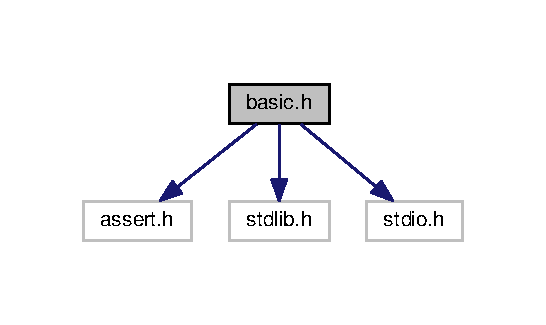
\includegraphics[width=262pt]{basic_8h__incl}
\end{center}
\end{figure}
This graph shows which files directly or indirectly include this file\+:
\nopagebreak
\begin{figure}[H]
\begin{center}
\leavevmode
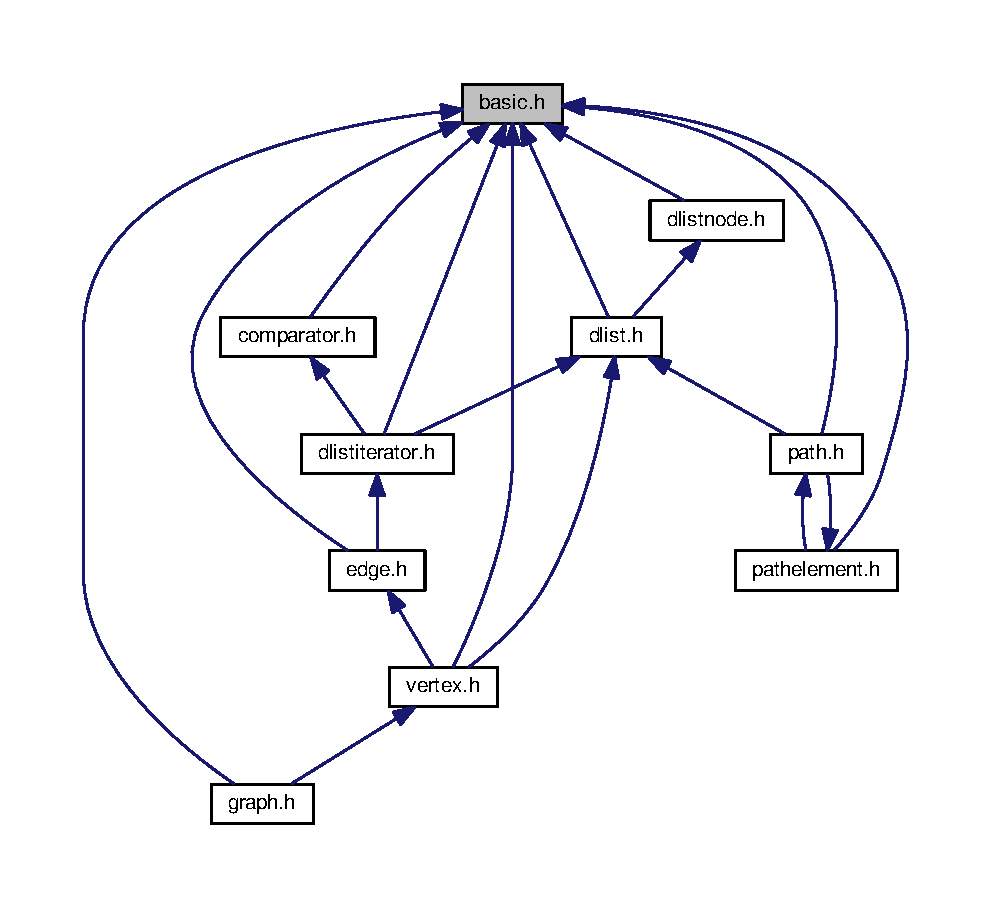
\includegraphics[width=350pt]{basic_8h__dep__incl}
\end{center}
\end{figure}
\subsection*{Typedefs}
\begin{DoxyCompactItemize}
\item 
typedef void $\ast$ \hyperlink{basic_8h_a5f051eaa796886555205c751e6d530f4}{Data}\hypertarget{basic_8h_a5f051eaa796886555205c751e6d530f4}{}\label{basic_8h_a5f051eaa796886555205c751e6d530f4}

\begin{DoxyCompactList}\small\item\em Typedefing \textquotesingle{}void $\ast$\textquotesingle{} to Data for better readablility. \end{DoxyCompactList}\end{DoxyCompactItemize}
\subsection*{Enumerations}
\begin{DoxyCompactItemize}
\item 
enum {\bfseries bool} \{ {\bfseries false} = 0, 
{\bfseries true} = !false
 \}\hypertarget{basic_8h_af6a258d8f3ee5206d682d799316314b1}{}\label{basic_8h_af6a258d8f3ee5206d682d799316314b1}

\end{DoxyCompactItemize}


\subsection{Detailed Description}
Just some arbitrary definitions for the library. 

\begin{DoxyAuthor}{Author}
Philipp Badenhoop 
\end{DoxyAuthor}
\begin{DoxyDate}{Date}
6 Jun 2016 
\end{DoxyDate}

\hypertarget{comparator_8h}{}\section{comparator.\+h File Reference}
\label{comparator_8h}\index{comparator.\+h@{comparator.\+h}}


An object to compare data. As an example, it can be used to search data in a list.  


{\ttfamily \#include \char`\"{}basic.\+h\char`\"{}}\\*
Include dependency graph for comparator.\+h\+:\nopagebreak
\begin{figure}[H]
\begin{center}
\leavevmode
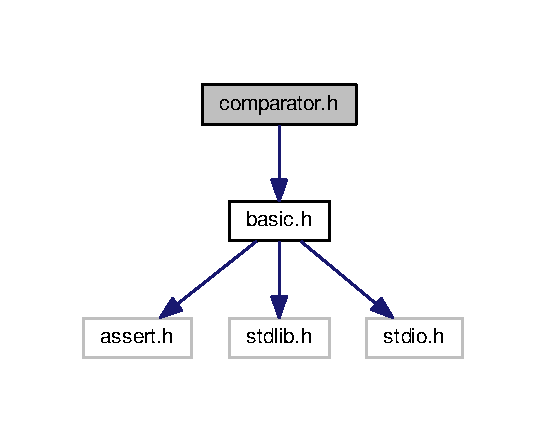
\includegraphics[width=262pt]{comparator_8h__incl}
\end{center}
\end{figure}
This graph shows which files directly or indirectly include this file\+:\nopagebreak
\begin{figure}[H]
\begin{center}
\leavevmode
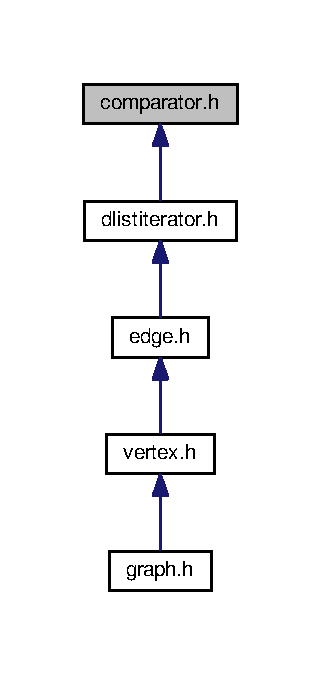
\includegraphics[width=154pt]{comparator_8h__dep__incl}
\end{center}
\end{figure}
\subsection*{Data Structures}
\begin{DoxyCompactItemize}
\item 
struct \hyperlink{structComparator}{Comparator}
\begin{DoxyCompactList}\small\item\em An object to compare data. \end{DoxyCompactList}\end{DoxyCompactItemize}
\subsection*{Typedefs}
\begin{DoxyCompactItemize}
\item 
typedef bool($\ast$ \hyperlink{comparator_8h_a7031dbbb6ddea05773826b8d54940494}{Compare\+Function}) (\hyperlink{basic_8h_a5f051eaa796886555205c751e6d530f4}{Data}, \hyperlink{basic_8h_a5f051eaa796886555205c751e6d530f4}{Data})\hypertarget{comparator_8h_a7031dbbb6ddea05773826b8d54940494}{}\label{comparator_8h_a7031dbbb6ddea05773826b8d54940494}

\begin{DoxyCompactList}\small\item\em A function comparing data. It returns true, if the data is matching the implemented compare criteria. \end{DoxyCompactList}\end{DoxyCompactItemize}
\subsection*{Functions}
\begin{DoxyCompactItemize}
\item 
\hyperlink{structComparator}{Comparator} $\ast$ \hyperlink{comparator_8h_a86ed76bd8254ed436dac0cdc1e895b9f}{comparator\+\_\+new} (\hyperlink{basic_8h_a5f051eaa796886555205c751e6d530f4}{Data} data, \hyperlink{comparator_8h_a7031dbbb6ddea05773826b8d54940494}{Compare\+Function} compare\+Function)
\begin{DoxyCompactList}\small\item\em Allocates and initializes a new comparator. \end{DoxyCompactList}\item 
void \hyperlink{comparator_8h_a71bb7e96b7288c97e84aee0f34e615eb}{comparator\+\_\+destroy} (\hyperlink{structComparator}{Comparator} $\ast$)\hypertarget{comparator_8h_a71bb7e96b7288c97e84aee0f34e615eb}{}\label{comparator_8h_a71bb7e96b7288c97e84aee0f34e615eb}

\begin{DoxyCompactList}\small\item\em Simply frees the comparator. \end{DoxyCompactList}\item 
bool \hyperlink{comparator_8h_a4034151cc627c0df520968295c64beff}{comparator\+\_\+compare} (\hyperlink{structComparator}{Comparator} $\ast$, \hyperlink{basic_8h_a5f051eaa796886555205c751e6d530f4}{Data})
\begin{DoxyCompactList}\small\item\em Compares the stored data with input data. \end{DoxyCompactList}\end{DoxyCompactItemize}


\subsection{Detailed Description}
An object to compare data. As an example, it can be used to search data in a list. 

\begin{DoxyAuthor}{Author}
Philipp Badenhoop 
\end{DoxyAuthor}
\begin{DoxyDate}{Date}
4 Jun 2016 
\end{DoxyDate}


\subsection{Function Documentation}
\index{comparator.\+h@{comparator.\+h}!comparator\+\_\+compare@{comparator\+\_\+compare}}
\index{comparator\+\_\+compare@{comparator\+\_\+compare}!comparator.\+h@{comparator.\+h}}
\subsubsection[{\texorpdfstring{comparator\+\_\+compare(\+Comparator $\ast$, Data)}{comparator_compare(Comparator *, Data)}}]{\setlength{\rightskip}{0pt plus 5cm}bool comparator\+\_\+compare (
\begin{DoxyParamCaption}
\item[{{\bf Comparator} $\ast$}]{, }
\item[{{\bf Data}}]{}
\end{DoxyParamCaption}
)}\hypertarget{comparator_8h_a4034151cc627c0df520968295c64beff}{}\label{comparator_8h_a4034151cc627c0df520968295c64beff}


Compares the stored data with input data. 

\begin{DoxyReturn}{Returns}
true, if the stored and input data match the implemented compare criteria. 
\end{DoxyReturn}
\index{comparator.\+h@{comparator.\+h}!comparator\+\_\+new@{comparator\+\_\+new}}
\index{comparator\+\_\+new@{comparator\+\_\+new}!comparator.\+h@{comparator.\+h}}
\subsubsection[{\texorpdfstring{comparator\+\_\+new(\+Data data, Compare\+Function compare\+Function)}{comparator_new(Data data, CompareFunction compareFunction)}}]{\setlength{\rightskip}{0pt plus 5cm}{\bf Comparator}$\ast$ comparator\+\_\+new (
\begin{DoxyParamCaption}
\item[{{\bf Data}}]{data, }
\item[{{\bf Compare\+Function}}]{compare\+Function}
\end{DoxyParamCaption}
)}\hypertarget{comparator_8h_a86ed76bd8254ed436dac0cdc1e895b9f}{}\label{comparator_8h_a86ed76bd8254ed436dac0cdc1e895b9f}


Allocates and initializes a new comparator. 


\begin{DoxyParams}{Parameters}
{\em data} & \\
\hline
{\em compare\+Function} & \\
\hline
\end{DoxyParams}
\begin{DoxyReturn}{Returns}
The pointer to the new comparator. 
\end{DoxyReturn}

\hypertarget{dlist_8h}{}\section{dlist.\+h File Reference}
\label{dlist_8h}\index{dlist.\+h@{dlist.\+h}}


A generic doubly linked list.  


{\ttfamily \#include \char`\"{}basic.\+h\char`\"{}}\\*
{\ttfamily \#include \char`\"{}dlistnode.\+h\char`\"{}}\\*
Include dependency graph for dlist.\+h\+:\nopagebreak
\begin{figure}[H]
\begin{center}
\leavevmode
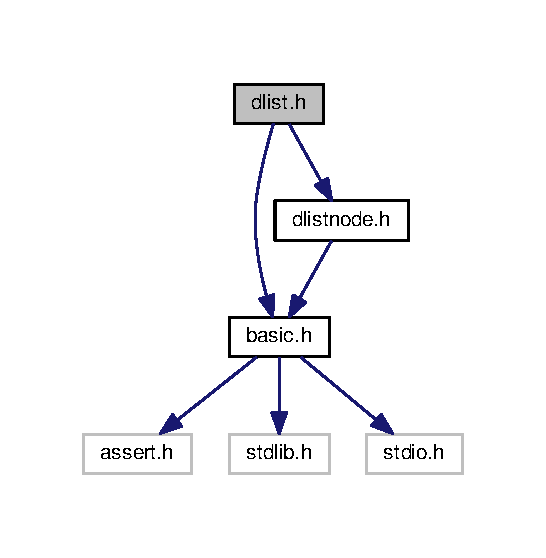
\includegraphics[width=262pt]{dlist_8h__incl}
\end{center}
\end{figure}
This graph shows which files directly or indirectly include this file\+:
\nopagebreak
\begin{figure}[H]
\begin{center}
\leavevmode
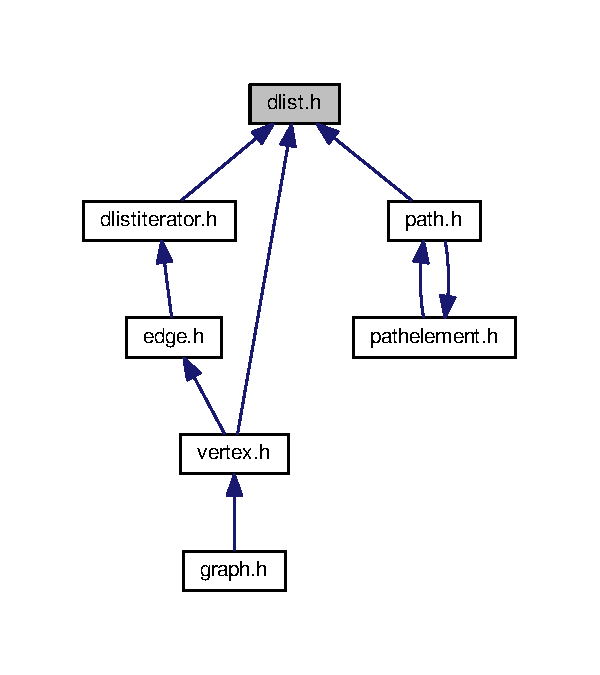
\includegraphics[width=288pt]{dlist_8h__dep__incl}
\end{center}
\end{figure}
\subsection*{Data Structures}
\begin{DoxyCompactItemize}
\item 
struct \hyperlink{structDList}{D\+List}
\begin{DoxyCompactList}\small\item\em The data structure of a generic doubly linked list. \end{DoxyCompactList}\end{DoxyCompactItemize}
\subsection*{Typedefs}
\begin{DoxyCompactItemize}
\item 
typedef void($\ast$ \hyperlink{dlist_8h_a2206207e78cb6335a8f41ad6cf76b55c}{Destroy\+Function}) (\hyperlink{basic_8h_a5f051eaa796886555205c751e6d530f4}{Data})\hypertarget{dlist_8h_a2206207e78cb6335a8f41ad6cf76b55c}{}\label{dlist_8h_a2206207e78cb6335a8f41ad6cf76b55c}

\begin{DoxyCompactList}\small\item\em A pointer to a function which destroys the generic data. \end{DoxyCompactList}\end{DoxyCompactItemize}
\subsection*{Functions}
\begin{DoxyCompactItemize}
\item 
\hyperlink{structDList}{D\+List} $\ast$ \hyperlink{dlist_8h_a4345525d397ca8b568beb853c4486f51}{d\+List\+\_\+new} (int element\+Size, \hyperlink{dlist_8h_a2206207e78cb6335a8f41ad6cf76b55c}{Destroy\+Function} destroy\+Function)
\begin{DoxyCompactList}\small\item\em Allocates and initializes a new list. It also creates the discrete begin and end node. \end{DoxyCompactList}\item 
void \hyperlink{dlist_8h_a9c3f8ad5e49b5c2379cddc20823dbad0}{d\+List\+\_\+destroy} (\hyperlink{structDList}{D\+List} $\ast$list)
\begin{DoxyCompactList}\small\item\em Simply frees the pointer to the list. \end{DoxyCompactList}\item 
void \hyperlink{dlist_8h_a60eeb1c2d0a580852c091c6c8cb5d3fd}{d\+List\+\_\+destroy\+All} (\hyperlink{structDList}{D\+List} $\ast$list)
\begin{DoxyCompactList}\small\item\em Completely destroys and frees the list, including its nodes and their data. \end{DoxyCompactList}\item 
int \hyperlink{dlist_8h_a295d8e7a2055925c35f9ee530e387cc5}{d\+List\+\_\+get\+Size} (\hyperlink{structDList}{D\+List} $\ast$list)
\item 
bool \hyperlink{dlist_8h_af16b1e6b4d0d278ecf6baf8e57ee41bc}{d\+List\+\_\+is\+Empty} (\hyperlink{structDList}{D\+List} $\ast$list)
\item 
void \hyperlink{dlist_8h_ab695f8f645ad8da47614aa8cdab9ec16}{d\+List\+\_\+append} (\hyperlink{structDList}{D\+List} $\ast$list, \hyperlink{basic_8h_a5f051eaa796886555205c751e6d530f4}{Data} data)
\begin{DoxyCompactList}\small\item\em Inserts a new node whichs stores given data after the last node of the list. \end{DoxyCompactList}\item 
\hyperlink{basic_8h_a5f051eaa796886555205c751e6d530f4}{Data} \hyperlink{dlist_8h_ab79c5b74e3e2d7d589f9b4c00d7e7754}{d\+List\+\_\+get} (\hyperlink{structDList}{D\+List} $\ast$list, int i)
\end{DoxyCompactItemize}


\subsection{Detailed Description}
A generic doubly linked list. 

\begin{DoxyAuthor}{Author}
Philipp Badenhoop 
\end{DoxyAuthor}
\begin{DoxyDate}{Date}
4 Jun 2016 
\end{DoxyDate}


\subsection{Function Documentation}
\index{dlist.\+h@{dlist.\+h}!d\+List\+\_\+append@{d\+List\+\_\+append}}
\index{d\+List\+\_\+append@{d\+List\+\_\+append}!dlist.\+h@{dlist.\+h}}
\subsubsection[{\texorpdfstring{d\+List\+\_\+append(\+D\+List $\ast$list, Data data)}{dList_append(DList *list, Data data)}}]{\setlength{\rightskip}{0pt plus 5cm}void d\+List\+\_\+append (
\begin{DoxyParamCaption}
\item[{{\bf D\+List} $\ast$}]{list, }
\item[{{\bf Data}}]{data}
\end{DoxyParamCaption}
)}\hypertarget{dlist_8h_ab695f8f645ad8da47614aa8cdab9ec16}{}\label{dlist_8h_ab695f8f645ad8da47614aa8cdab9ec16}


Inserts a new node whichs stores given data after the last node of the list. 


\begin{DoxyParams}{Parameters}
{\em list} & \\
\hline
{\em data} & The data which the new node will be storing. \\
\hline
\end{DoxyParams}
\index{dlist.\+h@{dlist.\+h}!d\+List\+\_\+destroy@{d\+List\+\_\+destroy}}
\index{d\+List\+\_\+destroy@{d\+List\+\_\+destroy}!dlist.\+h@{dlist.\+h}}
\subsubsection[{\texorpdfstring{d\+List\+\_\+destroy(\+D\+List $\ast$list)}{dList_destroy(DList *list)}}]{\setlength{\rightskip}{0pt plus 5cm}void d\+List\+\_\+destroy (
\begin{DoxyParamCaption}
\item[{{\bf D\+List} $\ast$}]{list}
\end{DoxyParamCaption}
)}\hypertarget{dlist_8h_a9c3f8ad5e49b5c2379cddc20823dbad0}{}\label{dlist_8h_a9c3f8ad5e49b5c2379cddc20823dbad0}


Simply frees the pointer to the list. 


\begin{DoxyParams}{Parameters}
{\em list} & \\
\hline
\end{DoxyParams}
\index{dlist.\+h@{dlist.\+h}!d\+List\+\_\+destroy\+All@{d\+List\+\_\+destroy\+All}}
\index{d\+List\+\_\+destroy\+All@{d\+List\+\_\+destroy\+All}!dlist.\+h@{dlist.\+h}}
\subsubsection[{\texorpdfstring{d\+List\+\_\+destroy\+All(\+D\+List $\ast$list)}{dList_destroyAll(DList *list)}}]{\setlength{\rightskip}{0pt plus 5cm}void d\+List\+\_\+destroy\+All (
\begin{DoxyParamCaption}
\item[{{\bf D\+List} $\ast$}]{list}
\end{DoxyParamCaption}
)}\hypertarget{dlist_8h_a60eeb1c2d0a580852c091c6c8cb5d3fd}{}\label{dlist_8h_a60eeb1c2d0a580852c091c6c8cb5d3fd}


Completely destroys and frees the list, including its nodes and their data. 


\begin{DoxyParams}{Parameters}
{\em list} & \\
\hline
\end{DoxyParams}
\index{dlist.\+h@{dlist.\+h}!d\+List\+\_\+get@{d\+List\+\_\+get}}
\index{d\+List\+\_\+get@{d\+List\+\_\+get}!dlist.\+h@{dlist.\+h}}
\subsubsection[{\texorpdfstring{d\+List\+\_\+get(\+D\+List $\ast$list, int i)}{dList_get(DList *list, int i)}}]{\setlength{\rightskip}{0pt plus 5cm}{\bf Data} d\+List\+\_\+get (
\begin{DoxyParamCaption}
\item[{{\bf D\+List} $\ast$}]{list, }
\item[{int}]{i}
\end{DoxyParamCaption}
)}\hypertarget{dlist_8h_ab79c5b74e3e2d7d589f9b4c00d7e7754}{}\label{dlist_8h_ab79c5b74e3e2d7d589f9b4c00d7e7754}

\begin{DoxyParams}{Parameters}
{\em list} & \\
\hline
{\em i} & \\
\hline
\end{DoxyParams}
\begin{DoxyReturn}{Returns}
The data of the i-\/th node of the list (start counting at the first node). 
\end{DoxyReturn}
\index{dlist.\+h@{dlist.\+h}!d\+List\+\_\+get\+Size@{d\+List\+\_\+get\+Size}}
\index{d\+List\+\_\+get\+Size@{d\+List\+\_\+get\+Size}!dlist.\+h@{dlist.\+h}}
\subsubsection[{\texorpdfstring{d\+List\+\_\+get\+Size(\+D\+List $\ast$list)}{dList_getSize(DList *list)}}]{\setlength{\rightskip}{0pt plus 5cm}int d\+List\+\_\+get\+Size (
\begin{DoxyParamCaption}
\item[{{\bf D\+List} $\ast$}]{list}
\end{DoxyParamCaption}
)}\hypertarget{dlist_8h_a295d8e7a2055925c35f9ee530e387cc5}{}\label{dlist_8h_a295d8e7a2055925c35f9ee530e387cc5}

\begin{DoxyParams}{Parameters}
{\em list} & \\
\hline
\end{DoxyParams}
\begin{DoxyReturn}{Returns}
The number of nodes in the list excluding the discrete begin and end nodes. 
\end{DoxyReturn}
\index{dlist.\+h@{dlist.\+h}!d\+List\+\_\+is\+Empty@{d\+List\+\_\+is\+Empty}}
\index{d\+List\+\_\+is\+Empty@{d\+List\+\_\+is\+Empty}!dlist.\+h@{dlist.\+h}}
\subsubsection[{\texorpdfstring{d\+List\+\_\+is\+Empty(\+D\+List $\ast$list)}{dList_isEmpty(DList *list)}}]{\setlength{\rightskip}{0pt plus 5cm}bool d\+List\+\_\+is\+Empty (
\begin{DoxyParamCaption}
\item[{{\bf D\+List} $\ast$}]{list}
\end{DoxyParamCaption}
)}\hypertarget{dlist_8h_af16b1e6b4d0d278ecf6baf8e57ee41bc}{}\label{dlist_8h_af16b1e6b4d0d278ecf6baf8e57ee41bc}

\begin{DoxyParams}{Parameters}
{\em list} & \\
\hline
\end{DoxyParams}
\begin{DoxyReturn}{Returns}
true, if there\textquotesingle{}re no nodes in the list except the discrete begin and end nodes. 
\end{DoxyReturn}
\index{dlist.\+h@{dlist.\+h}!d\+List\+\_\+new@{d\+List\+\_\+new}}
\index{d\+List\+\_\+new@{d\+List\+\_\+new}!dlist.\+h@{dlist.\+h}}
\subsubsection[{\texorpdfstring{d\+List\+\_\+new(int element\+Size, Destroy\+Function destroy\+Function)}{dList_new(int elementSize, DestroyFunction destroyFunction)}}]{\setlength{\rightskip}{0pt plus 5cm}{\bf D\+List}$\ast$ d\+List\+\_\+new (
\begin{DoxyParamCaption}
\item[{int}]{element\+Size, }
\item[{{\bf Destroy\+Function}}]{destroy\+Function}
\end{DoxyParamCaption}
)}\hypertarget{dlist_8h_a4345525d397ca8b568beb853c4486f51}{}\label{dlist_8h_a4345525d397ca8b568beb853c4486f51}


Allocates and initializes a new list. It also creates the discrete begin and end node. 


\begin{DoxyParams}{Parameters}
{\em element\+Size} & The size of the data stored in each node. \\
\hline
{\em Destroy\+Function} & A function which destroys the data of a node. \\
\hline
\end{DoxyParams}
\begin{DoxyReturn}{Returns}
A pointer to the created list. 
\end{DoxyReturn}

\hypertarget{dlistiterator_8h}{}\section{dlistiterator.\+h File Reference}
\label{dlistiterator_8h}\index{dlistiterator.\+h@{dlistiterator.\+h}}


A bidirectional iterator for a doubly linked list.  


{\ttfamily \#include \char`\"{}basic.\+h\char`\"{}}\\*
{\ttfamily \#include \char`\"{}dlist.\+h\char`\"{}}\\*
{\ttfamily \#include \char`\"{}comparator.\+h\char`\"{}}\\*
Include dependency graph for dlistiterator.\+h\+:
\nopagebreak
\begin{figure}[H]
\begin{center}
\leavevmode
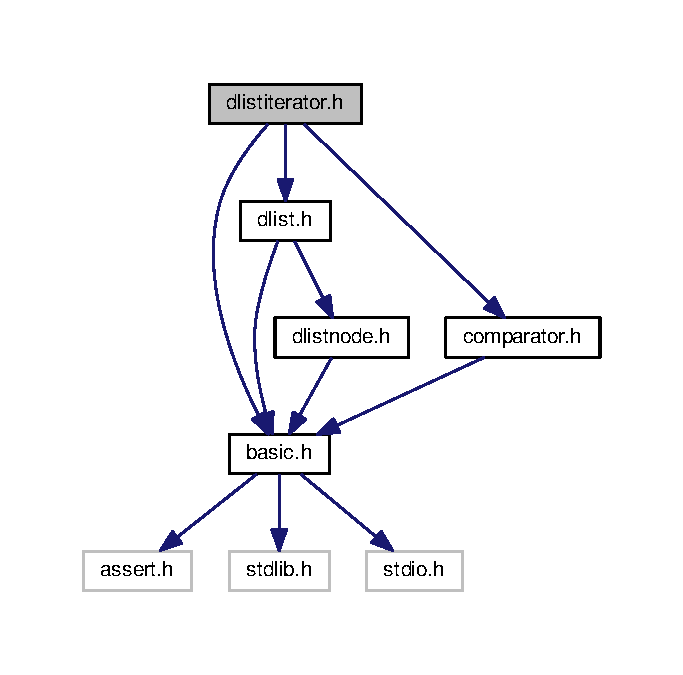
\includegraphics[width=328pt]{dlistiterator_8h__incl}
\end{center}
\end{figure}
This graph shows which files directly or indirectly include this file\+:
\nopagebreak
\begin{figure}[H]
\begin{center}
\leavevmode
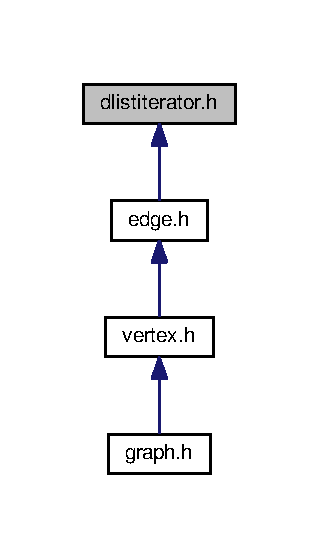
\includegraphics[width=153pt]{dlistiterator_8h__dep__incl}
\end{center}
\end{figure}
\subsection*{Data Structures}
\begin{DoxyCompactItemize}
\item 
struct \hyperlink{structDListIterator}{D\+List\+Iterator}
\begin{DoxyCompactList}\small\item\em A simple bidirectional iterator. \end{DoxyCompactList}\end{DoxyCompactItemize}
\subsection*{Macros}
\begin{DoxyCompactItemize}
\item 
\#define \hyperlink{dlistiterator_8h_a6ae949a09312f851d5a1d80f4db0211d}{d\+List\+\_\+foreach}(iterator)
\begin{DoxyCompactList}\small\item\em With the \hyperlink{structDListIterator}{D\+List\+Iterator} you can simply mimic a foreach loop. It iterates through each node in the list starting with the first node and ending on the discrete end node. \end{DoxyCompactList}\item 
\#define \hyperlink{dlistiterator_8h_abd85458a77df0ac281983e3e6e5eec29}{d\+List\+\_\+foreach\+Down}(iterator)
\begin{DoxyCompactList}\small\item\em With the \hyperlink{structDListIterator}{D\+List\+Iterator} you can simply mimic a foreach loop. It iterates through each node in the list starting with the last node and ending on the discrete begin node. \end{DoxyCompactList}\end{DoxyCompactItemize}
\subsection*{Functions}
\begin{DoxyCompactItemize}
\item 
\hyperlink{structDListIterator}{D\+List\+Iterator} $\ast$ \hyperlink{dlistiterator_8h_a8c6fe318a1fd55f6f588f9fb9d1f95fb}{d\+List\+Iterator\+\_\+new} (\hyperlink{structDList}{D\+List} $\ast$list)
\begin{DoxyCompactList}\small\item\em Allocates and initializes a new iterator. \end{DoxyCompactList}\item 
void \hyperlink{dlistiterator_8h_a9cdeec2250f90a60c8e4866b4ecff8fc}{d\+List\+Iterator\+\_\+destroy} (\hyperlink{structDListIterator}{D\+List\+Iterator} $\ast$iterator)
\begin{DoxyCompactList}\small\item\em Simply frees the pointer to the iterator. \end{DoxyCompactList}\item 
void \hyperlink{dlistiterator_8h_a9b284f631ebd355706fbf4939c2d70bf}{d\+List\+Iterator\+\_\+increment} (\hyperlink{structDListIterator}{D\+List\+Iterator} $\ast$iterator)
\begin{DoxyCompactList}\small\item\em The current node is set to its next node. \end{DoxyCompactList}\item 
void \hyperlink{dlistiterator_8h_aecc3cba721cabfe6e99c9426e386795c}{d\+List\+Iterator\+\_\+decrement} (\hyperlink{structDListIterator}{D\+List\+Iterator} $\ast$iterator)
\begin{DoxyCompactList}\small\item\em The current node is set to its previous node. \end{DoxyCompactList}\item 
bool \hyperlink{dlistiterator_8h_a906e71ecbed84905246acd0f3f0a737b}{d\+List\+Iterator\+\_\+is\+At\+End} (\hyperlink{structDListIterator}{D\+List\+Iterator} $\ast$iterator)
\item 
bool \hyperlink{dlistiterator_8h_a18e7ea340620815e7fec089948286a88}{d\+List\+Iterator\+\_\+is\+At\+Begin} (\hyperlink{structDListIterator}{D\+List\+Iterator} $\ast$iterator)
\item 
void \hyperlink{dlistiterator_8h_a04960af0164fc5ad14a8a650ca11a59f}{d\+List\+Iterator\+\_\+insert\+After} (\hyperlink{structDListIterator}{D\+List\+Iterator} $\ast$iterator, \hyperlink{basic_8h_a5f051eaa796886555205c751e6d530f4}{Data} data)
\begin{DoxyCompactList}\small\item\em Inserts a new node with given data between the current node and the next node of the current node. \end{DoxyCompactList}\item 
void \hyperlink{dlistiterator_8h_ae5e4c00bd3f2b7a85c6f38e5731d235e}{d\+List\+Iterator\+\_\+remove} (\hyperlink{structDListIterator}{D\+List\+Iterator} $\ast$iterator)
\begin{DoxyCompactList}\small\item\em Destroys the current node and reconnects the nodes. \end{DoxyCompactList}\item 
void \hyperlink{dlistiterator_8h_a887053dafcab55a79ce65ed6a820909c}{d\+List\+Iterator\+\_\+remove\+And\+Destroy} (\hyperlink{structDListIterator}{D\+List\+Iterator} $\ast$iterator)
\begin{DoxyCompactList}\small\item\em Destroy the current node, reconnects the nodes and also destroys the data of the current node. \end{DoxyCompactList}\item 
\hyperlink{basic_8h_a5f051eaa796886555205c751e6d530f4}{Data} \hyperlink{dlistiterator_8h_ae2f4cb30c14a94da1c843ba79bd418b2}{d\+List\+Iterator\+\_\+get} (\hyperlink{structDListIterator}{D\+List\+Iterator} $\ast$iterator)
\item 
\hyperlink{basic_8h_a5f051eaa796886555205c751e6d530f4}{Data} \hyperlink{dlistiterator_8h_a6bfe7399f641f4dcdd54212f4b3a268f}{d\+List\+Iterator\+\_\+search} (\hyperlink{structDListIterator}{D\+List\+Iterator} $\ast$iterator, \hyperlink{structComparator}{Comparator} $\ast$comparator)
\begin{DoxyCompactList}\small\item\em Uses a comparator object to search a node in the list. The search is incremental and starts at the current node. \end{DoxyCompactList}\item 
void \hyperlink{dlistiterator_8h_afde985be14b96579309b54eed487edd6}{d\+List\+Iterator\+\_\+to\+First} (\hyperlink{structDListIterator}{D\+List\+Iterator} $\ast$iterator)
\begin{DoxyCompactList}\small\item\em Sets the current node to the {\bfseries first} node of the list. \end{DoxyCompactList}\item 
void \hyperlink{dlistiterator_8h_aa5fb3cc3e82ba75af115999bccd88460}{d\+List\+Iterator\+\_\+to\+Last} (\hyperlink{structDListIterator}{D\+List\+Iterator} $\ast$iterator)
\begin{DoxyCompactList}\small\item\em Sets the current node to the {\bfseries last} node of the lsit. \end{DoxyCompactList}\item 
void \hyperlink{dlistiterator_8h_a771716dfe7506ec19eeae3f5dbd8efca}{d\+List\+Iterator\+\_\+merge} (\hyperlink{structDListIterator}{D\+List\+Iterator} $\ast$iterator, \hyperlink{structDList}{D\+List} $\ast$merge\+List)
\begin{DoxyCompactList}\small\item\em Inserts the nodes of the specified merge list (excluding the discrete begin and end nodes) after the current node. \end{DoxyCompactList}\end{DoxyCompactItemize}


\subsection{Detailed Description}
A bidirectional iterator for a doubly linked list. 

\begin{DoxyAuthor}{Author}
Philipp Badenhoop 
\end{DoxyAuthor}
\begin{DoxyDate}{Date}
6 Jun 2016 
\end{DoxyDate}


\subsection{Macro Definition Documentation}
\index{dlistiterator.\+h@{dlistiterator.\+h}!d\+List\+\_\+foreach@{d\+List\+\_\+foreach}}
\index{d\+List\+\_\+foreach@{d\+List\+\_\+foreach}!dlistiterator.\+h@{dlistiterator.\+h}}
\subsubsection[{\texorpdfstring{d\+List\+\_\+foreach}{dList_foreach}}]{\setlength{\rightskip}{0pt plus 5cm}\#define d\+List\+\_\+foreach(
\begin{DoxyParamCaption}
\item[{}]{iterator}
\end{DoxyParamCaption}
)}\hypertarget{dlistiterator_8h_a6ae949a09312f851d5a1d80f4db0211d}{}\label{dlistiterator_8h_a6ae949a09312f851d5a1d80f4db0211d}
{\bfseries Value\+:}
\begin{DoxyCode}
\textcolor{keywordflow}{for}( \hyperlink{dlistiterator_8h_afde985be14b96579309b54eed487edd6}{dListIterator\_toFirst}( iterator ); \(\backslash\)
                                         !\hyperlink{dlistiterator_8h_a906e71ecbed84905246acd0f3f0a737b}{dListIterator\_isAtEnd}( iterator ); 
      \hyperlink{dlistiterator_8h_a9b284f631ebd355706fbf4939c2d70bf}{\(\backslash\)}
\hyperlink{dlistiterator_8h_a9b284f631ebd355706fbf4939c2d70bf}{                                         dListIterator\_increment}
      ( iterator ))
\end{DoxyCode}


With the \hyperlink{structDListIterator}{D\+List\+Iterator} you can simply mimic a foreach loop. It iterates through each node in the list starting with the first node and ending on the discrete end node. 

\begin{DoxyAttention}{Attention}
When the loop is over, the iterator stands on the discrete end node. This means\+: If you want to get the data of the current node afterwards, you {\bfseries must} set the iterator to a valid node first (not the discrete begin or end nodes)! 
\end{DoxyAttention}
\index{dlistiterator.\+h@{dlistiterator.\+h}!d\+List\+\_\+foreach\+Down@{d\+List\+\_\+foreach\+Down}}
\index{d\+List\+\_\+foreach\+Down@{d\+List\+\_\+foreach\+Down}!dlistiterator.\+h@{dlistiterator.\+h}}
\subsubsection[{\texorpdfstring{d\+List\+\_\+foreach\+Down}{dList_foreachDown}}]{\setlength{\rightskip}{0pt plus 5cm}\#define d\+List\+\_\+foreach\+Down(
\begin{DoxyParamCaption}
\item[{}]{iterator}
\end{DoxyParamCaption}
)}\hypertarget{dlistiterator_8h_abd85458a77df0ac281983e3e6e5eec29}{}\label{dlistiterator_8h_abd85458a77df0ac281983e3e6e5eec29}
{\bfseries Value\+:}
\begin{DoxyCode}
\textcolor{keywordflow}{for}( \hyperlink{dlistiterator_8h_aa5fb3cc3e82ba75af115999bccd88460}{dListIterator\_toLast}( iterator ); \(\backslash\)
                                             !\hyperlink{dlistiterator_8h_a18e7ea340620815e7fec089948286a88}{dListIterator\_isAtBegin}( iterator ); 
      \hyperlink{dlistiterator_8h_aecc3cba721cabfe6e99c9426e386795c}{\(\backslash\)}
\hyperlink{dlistiterator_8h_aecc3cba721cabfe6e99c9426e386795c}{                                             dListIterator\_decrement}
      ( iterator ))
\end{DoxyCode}


With the \hyperlink{structDListIterator}{D\+List\+Iterator} you can simply mimic a foreach loop. It iterates through each node in the list starting with the last node and ending on the discrete begin node. 

\begin{DoxyAttention}{Attention}
When the loop is over, the iterator stands on the discrete begin node. This means\+: If you want to get the data of the current node afterwards, you {\bfseries must} set the iterator to a valid node first (not the discrete begin or end nodes)! 
\end{DoxyAttention}


\subsection{Function Documentation}
\index{dlistiterator.\+h@{dlistiterator.\+h}!d\+List\+Iterator\+\_\+decrement@{d\+List\+Iterator\+\_\+decrement}}
\index{d\+List\+Iterator\+\_\+decrement@{d\+List\+Iterator\+\_\+decrement}!dlistiterator.\+h@{dlistiterator.\+h}}
\subsubsection[{\texorpdfstring{d\+List\+Iterator\+\_\+decrement(\+D\+List\+Iterator $\ast$iterator)}{dListIterator_decrement(DListIterator *iterator)}}]{\setlength{\rightskip}{0pt plus 5cm}void d\+List\+Iterator\+\_\+decrement (
\begin{DoxyParamCaption}
\item[{{\bf D\+List\+Iterator} $\ast$}]{iterator}
\end{DoxyParamCaption}
)}\hypertarget{dlistiterator_8h_aecc3cba721cabfe6e99c9426e386795c}{}\label{dlistiterator_8h_aecc3cba721cabfe6e99c9426e386795c}


The current node is set to its previous node. 


\begin{DoxyParams}{Parameters}
{\em iterator} & \\
\hline
\end{DoxyParams}
\begin{DoxyAttention}{Attention}
Do not decrement if the current node is the discrete begin node! 
\end{DoxyAttention}
\index{dlistiterator.\+h@{dlistiterator.\+h}!d\+List\+Iterator\+\_\+destroy@{d\+List\+Iterator\+\_\+destroy}}
\index{d\+List\+Iterator\+\_\+destroy@{d\+List\+Iterator\+\_\+destroy}!dlistiterator.\+h@{dlistiterator.\+h}}
\subsubsection[{\texorpdfstring{d\+List\+Iterator\+\_\+destroy(\+D\+List\+Iterator $\ast$iterator)}{dListIterator_destroy(DListIterator *iterator)}}]{\setlength{\rightskip}{0pt plus 5cm}void d\+List\+Iterator\+\_\+destroy (
\begin{DoxyParamCaption}
\item[{{\bf D\+List\+Iterator} $\ast$}]{iterator}
\end{DoxyParamCaption}
)}\hypertarget{dlistiterator_8h_a9cdeec2250f90a60c8e4866b4ecff8fc}{}\label{dlistiterator_8h_a9cdeec2250f90a60c8e4866b4ecff8fc}


Simply frees the pointer to the iterator. 


\begin{DoxyParams}{Parameters}
{\em iterator} & \\
\hline
\end{DoxyParams}
\index{dlistiterator.\+h@{dlistiterator.\+h}!d\+List\+Iterator\+\_\+get@{d\+List\+Iterator\+\_\+get}}
\index{d\+List\+Iterator\+\_\+get@{d\+List\+Iterator\+\_\+get}!dlistiterator.\+h@{dlistiterator.\+h}}
\subsubsection[{\texorpdfstring{d\+List\+Iterator\+\_\+get(\+D\+List\+Iterator $\ast$iterator)}{dListIterator_get(DListIterator *iterator)}}]{\setlength{\rightskip}{0pt plus 5cm}{\bf Data} d\+List\+Iterator\+\_\+get (
\begin{DoxyParamCaption}
\item[{{\bf D\+List\+Iterator} $\ast$}]{iterator}
\end{DoxyParamCaption}
)}\hypertarget{dlistiterator_8h_ae2f4cb30c14a94da1c843ba79bd418b2}{}\label{dlistiterator_8h_ae2f4cb30c14a94da1c843ba79bd418b2}

\begin{DoxyParams}{Parameters}
{\em iterator} & \\
\hline
\end{DoxyParams}
\begin{DoxyReturn}{Returns}
The data of the current node. 
\end{DoxyReturn}
\index{dlistiterator.\+h@{dlistiterator.\+h}!d\+List\+Iterator\+\_\+increment@{d\+List\+Iterator\+\_\+increment}}
\index{d\+List\+Iterator\+\_\+increment@{d\+List\+Iterator\+\_\+increment}!dlistiterator.\+h@{dlistiterator.\+h}}
\subsubsection[{\texorpdfstring{d\+List\+Iterator\+\_\+increment(\+D\+List\+Iterator $\ast$iterator)}{dListIterator_increment(DListIterator *iterator)}}]{\setlength{\rightskip}{0pt plus 5cm}void d\+List\+Iterator\+\_\+increment (
\begin{DoxyParamCaption}
\item[{{\bf D\+List\+Iterator} $\ast$}]{iterator}
\end{DoxyParamCaption}
)}\hypertarget{dlistiterator_8h_a9b284f631ebd355706fbf4939c2d70bf}{}\label{dlistiterator_8h_a9b284f631ebd355706fbf4939c2d70bf}


The current node is set to its next node. 


\begin{DoxyParams}{Parameters}
{\em iterator} & \\
\hline
\end{DoxyParams}
\begin{DoxyAttention}{Attention}
Do not increment if the current node is the discrete end node! 
\end{DoxyAttention}
\index{dlistiterator.\+h@{dlistiterator.\+h}!d\+List\+Iterator\+\_\+insert\+After@{d\+List\+Iterator\+\_\+insert\+After}}
\index{d\+List\+Iterator\+\_\+insert\+After@{d\+List\+Iterator\+\_\+insert\+After}!dlistiterator.\+h@{dlistiterator.\+h}}
\subsubsection[{\texorpdfstring{d\+List\+Iterator\+\_\+insert\+After(\+D\+List\+Iterator $\ast$iterator, Data data)}{dListIterator_insertAfter(DListIterator *iterator, Data data)}}]{\setlength{\rightskip}{0pt plus 5cm}void d\+List\+Iterator\+\_\+insert\+After (
\begin{DoxyParamCaption}
\item[{{\bf D\+List\+Iterator} $\ast$}]{iterator, }
\item[{{\bf Data}}]{data}
\end{DoxyParamCaption}
)}\hypertarget{dlistiterator_8h_a04960af0164fc5ad14a8a650ca11a59f}{}\label{dlistiterator_8h_a04960af0164fc5ad14a8a650ca11a59f}


Inserts a new node with given data between the current node and the next node of the current node. 


\begin{DoxyParams}{Parameters}
{\em iterator} & \\
\hline
{\em data} & \\
\hline
\end{DoxyParams}
\index{dlistiterator.\+h@{dlistiterator.\+h}!d\+List\+Iterator\+\_\+is\+At\+Begin@{d\+List\+Iterator\+\_\+is\+At\+Begin}}
\index{d\+List\+Iterator\+\_\+is\+At\+Begin@{d\+List\+Iterator\+\_\+is\+At\+Begin}!dlistiterator.\+h@{dlistiterator.\+h}}
\subsubsection[{\texorpdfstring{d\+List\+Iterator\+\_\+is\+At\+Begin(\+D\+List\+Iterator $\ast$iterator)}{dListIterator_isAtBegin(DListIterator *iterator)}}]{\setlength{\rightskip}{0pt plus 5cm}bool d\+List\+Iterator\+\_\+is\+At\+Begin (
\begin{DoxyParamCaption}
\item[{{\bf D\+List\+Iterator} $\ast$}]{iterator}
\end{DoxyParamCaption}
)}\hypertarget{dlistiterator_8h_a18e7ea340620815e7fec089948286a88}{}\label{dlistiterator_8h_a18e7ea340620815e7fec089948286a88}

\begin{DoxyParams}{Parameters}
{\em iterator} & \\
\hline
\end{DoxyParams}
\begin{DoxyReturn}{Returns}
true, if the current node is the {\bfseries discrete begin node} of the list.
\end{DoxyReturn}
\begin{DoxyAttention}{Attention}
It is not meant that the current node is the {\bfseries first node} of the list. Please check out the definitions of \hyperlink{structDList}{D\+List} for more information. 
\end{DoxyAttention}
\index{dlistiterator.\+h@{dlistiterator.\+h}!d\+List\+Iterator\+\_\+is\+At\+End@{d\+List\+Iterator\+\_\+is\+At\+End}}
\index{d\+List\+Iterator\+\_\+is\+At\+End@{d\+List\+Iterator\+\_\+is\+At\+End}!dlistiterator.\+h@{dlistiterator.\+h}}
\subsubsection[{\texorpdfstring{d\+List\+Iterator\+\_\+is\+At\+End(\+D\+List\+Iterator $\ast$iterator)}{dListIterator_isAtEnd(DListIterator *iterator)}}]{\setlength{\rightskip}{0pt plus 5cm}bool d\+List\+Iterator\+\_\+is\+At\+End (
\begin{DoxyParamCaption}
\item[{{\bf D\+List\+Iterator} $\ast$}]{iterator}
\end{DoxyParamCaption}
)}\hypertarget{dlistiterator_8h_a906e71ecbed84905246acd0f3f0a737b}{}\label{dlistiterator_8h_a906e71ecbed84905246acd0f3f0a737b}

\begin{DoxyParams}{Parameters}
{\em iterator} & \\
\hline
\end{DoxyParams}
\begin{DoxyReturn}{Returns}
true, if the current node is the {\bfseries discrete end node} of the list.
\end{DoxyReturn}
\begin{DoxyAttention}{Attention}
It is not meant that the current node is the {\bfseries last node} of the list. Please check out the definitions of \hyperlink{structDList}{D\+List} for more information. 
\end{DoxyAttention}
\index{dlistiterator.\+h@{dlistiterator.\+h}!d\+List\+Iterator\+\_\+merge@{d\+List\+Iterator\+\_\+merge}}
\index{d\+List\+Iterator\+\_\+merge@{d\+List\+Iterator\+\_\+merge}!dlistiterator.\+h@{dlistiterator.\+h}}
\subsubsection[{\texorpdfstring{d\+List\+Iterator\+\_\+merge(\+D\+List\+Iterator $\ast$iterator, D\+List $\ast$merge\+List)}{dListIterator_merge(DListIterator *iterator, DList *mergeList)}}]{\setlength{\rightskip}{0pt plus 5cm}void d\+List\+Iterator\+\_\+merge (
\begin{DoxyParamCaption}
\item[{{\bf D\+List\+Iterator} $\ast$}]{iterator, }
\item[{{\bf D\+List} $\ast$}]{merge\+List}
\end{DoxyParamCaption}
)}\hypertarget{dlistiterator_8h_a771716dfe7506ec19eeae3f5dbd8efca}{}\label{dlistiterator_8h_a771716dfe7506ec19eeae3f5dbd8efca}


Inserts the nodes of the specified merge list (excluding the discrete begin and end nodes) after the current node. 


\begin{DoxyParams}{Parameters}
{\em iterator} & \\
\hline
{\em merge\+List} & \\
\hline
\end{DoxyParams}
\begin{DoxyAttention}{Attention}
After doing this, it should be obvious that the merge list cannot be used anymore. Because of that, the merge list is going to be destroyed after calling this function! So do not access it anymore! 
\end{DoxyAttention}
\index{dlistiterator.\+h@{dlistiterator.\+h}!d\+List\+Iterator\+\_\+new@{d\+List\+Iterator\+\_\+new}}
\index{d\+List\+Iterator\+\_\+new@{d\+List\+Iterator\+\_\+new}!dlistiterator.\+h@{dlistiterator.\+h}}
\subsubsection[{\texorpdfstring{d\+List\+Iterator\+\_\+new(\+D\+List $\ast$list)}{dListIterator_new(DList *list)}}]{\setlength{\rightskip}{0pt plus 5cm}{\bf D\+List\+Iterator}$\ast$ d\+List\+Iterator\+\_\+new (
\begin{DoxyParamCaption}
\item[{{\bf D\+List} $\ast$}]{list}
\end{DoxyParamCaption}
)}\hypertarget{dlistiterator_8h_a8c6fe318a1fd55f6f588f9fb9d1f95fb}{}\label{dlistiterator_8h_a8c6fe318a1fd55f6f588f9fb9d1f95fb}


Allocates and initializes a new iterator. 


\begin{DoxyParams}{Parameters}
{\em list} & \\
\hline
\end{DoxyParams}
\begin{DoxyReturn}{Returns}
The pointer to the new iterator. 
\end{DoxyReturn}
\index{dlistiterator.\+h@{dlistiterator.\+h}!d\+List\+Iterator\+\_\+remove@{d\+List\+Iterator\+\_\+remove}}
\index{d\+List\+Iterator\+\_\+remove@{d\+List\+Iterator\+\_\+remove}!dlistiterator.\+h@{dlistiterator.\+h}}
\subsubsection[{\texorpdfstring{d\+List\+Iterator\+\_\+remove(\+D\+List\+Iterator $\ast$iterator)}{dListIterator_remove(DListIterator *iterator)}}]{\setlength{\rightskip}{0pt plus 5cm}void d\+List\+Iterator\+\_\+remove (
\begin{DoxyParamCaption}
\item[{{\bf D\+List\+Iterator} $\ast$}]{iterator}
\end{DoxyParamCaption}
)}\hypertarget{dlistiterator_8h_ae5e4c00bd3f2b7a85c6f38e5731d235e}{}\label{dlistiterator_8h_ae5e4c00bd3f2b7a85c6f38e5731d235e}


Destroys the current node and reconnects the nodes. 


\begin{DoxyParams}{Parameters}
{\em iterator} & \\
\hline
\end{DoxyParams}
\begin{DoxyAttention}{Attention}
This does not destroy the data of the current node! 
\end{DoxyAttention}
\index{dlistiterator.\+h@{dlistiterator.\+h}!d\+List\+Iterator\+\_\+remove\+And\+Destroy@{d\+List\+Iterator\+\_\+remove\+And\+Destroy}}
\index{d\+List\+Iterator\+\_\+remove\+And\+Destroy@{d\+List\+Iterator\+\_\+remove\+And\+Destroy}!dlistiterator.\+h@{dlistiterator.\+h}}
\subsubsection[{\texorpdfstring{d\+List\+Iterator\+\_\+remove\+And\+Destroy(\+D\+List\+Iterator $\ast$iterator)}{dListIterator_removeAndDestroy(DListIterator *iterator)}}]{\setlength{\rightskip}{0pt plus 5cm}void d\+List\+Iterator\+\_\+remove\+And\+Destroy (
\begin{DoxyParamCaption}
\item[{{\bf D\+List\+Iterator} $\ast$}]{iterator}
\end{DoxyParamCaption}
)}\hypertarget{dlistiterator_8h_a887053dafcab55a79ce65ed6a820909c}{}\label{dlistiterator_8h_a887053dafcab55a79ce65ed6a820909c}


Destroy the current node, reconnects the nodes and also destroys the data of the current node. 


\begin{DoxyParams}{Parameters}
{\em iterator} & \\
\hline
\end{DoxyParams}
\index{dlistiterator.\+h@{dlistiterator.\+h}!d\+List\+Iterator\+\_\+search@{d\+List\+Iterator\+\_\+search}}
\index{d\+List\+Iterator\+\_\+search@{d\+List\+Iterator\+\_\+search}!dlistiterator.\+h@{dlistiterator.\+h}}
\subsubsection[{\texorpdfstring{d\+List\+Iterator\+\_\+search(\+D\+List\+Iterator $\ast$iterator, Comparator $\ast$comparator)}{dListIterator_search(DListIterator *iterator, Comparator *comparator)}}]{\setlength{\rightskip}{0pt plus 5cm}{\bf Data} d\+List\+Iterator\+\_\+search (
\begin{DoxyParamCaption}
\item[{{\bf D\+List\+Iterator} $\ast$}]{iterator, }
\item[{{\bf Comparator} $\ast$}]{comparator}
\end{DoxyParamCaption}
)}\hypertarget{dlistiterator_8h_a6bfe7399f641f4dcdd54212f4b3a268f}{}\label{dlistiterator_8h_a6bfe7399f641f4dcdd54212f4b3a268f}


Uses a comparator object to search a node in the list. The search is incremental and starts at the current node. 


\begin{DoxyParams}{Parameters}
{\em iterator} & \\
\hline
{\em comparator} & \\
\hline
\end{DoxyParams}
\begin{DoxyReturn}{Returns}
The data of the node to search for if it finds it, else N\+U\+LL.
\end{DoxyReturn}
\begin{DoxyAttention}{Attention}
If it does not find the data to search for, the iterator\textquotesingle{}s current node will be the discrete end node. This means\+: If you want to get the data of the current node afterwards, you {\bfseries must} set the iterator to a valid node first (not the discrete begin or end nodes)! 
\end{DoxyAttention}
\index{dlistiterator.\+h@{dlistiterator.\+h}!d\+List\+Iterator\+\_\+to\+First@{d\+List\+Iterator\+\_\+to\+First}}
\index{d\+List\+Iterator\+\_\+to\+First@{d\+List\+Iterator\+\_\+to\+First}!dlistiterator.\+h@{dlistiterator.\+h}}
\subsubsection[{\texorpdfstring{d\+List\+Iterator\+\_\+to\+First(\+D\+List\+Iterator $\ast$iterator)}{dListIterator_toFirst(DListIterator *iterator)}}]{\setlength{\rightskip}{0pt plus 5cm}void d\+List\+Iterator\+\_\+to\+First (
\begin{DoxyParamCaption}
\item[{{\bf D\+List\+Iterator} $\ast$}]{iterator}
\end{DoxyParamCaption}
)}\hypertarget{dlistiterator_8h_afde985be14b96579309b54eed487edd6}{}\label{dlistiterator_8h_afde985be14b96579309b54eed487edd6}


Sets the current node to the {\bfseries first} node of the list. 


\begin{DoxyParams}{Parameters}
{\em iterator} & \\
\hline
\end{DoxyParams}
\begin{DoxyAttention}{Attention}
It is not meant that the current node will be set to the discrete begin node! Please check out the definitions of \hyperlink{structDList}{D\+List} for more information. 
\end{DoxyAttention}
\index{dlistiterator.\+h@{dlistiterator.\+h}!d\+List\+Iterator\+\_\+to\+Last@{d\+List\+Iterator\+\_\+to\+Last}}
\index{d\+List\+Iterator\+\_\+to\+Last@{d\+List\+Iterator\+\_\+to\+Last}!dlistiterator.\+h@{dlistiterator.\+h}}
\subsubsection[{\texorpdfstring{d\+List\+Iterator\+\_\+to\+Last(\+D\+List\+Iterator $\ast$iterator)}{dListIterator_toLast(DListIterator *iterator)}}]{\setlength{\rightskip}{0pt plus 5cm}void d\+List\+Iterator\+\_\+to\+Last (
\begin{DoxyParamCaption}
\item[{{\bf D\+List\+Iterator} $\ast$}]{iterator}
\end{DoxyParamCaption}
)}\hypertarget{dlistiterator_8h_aa5fb3cc3e82ba75af115999bccd88460}{}\label{dlistiterator_8h_aa5fb3cc3e82ba75af115999bccd88460}


Sets the current node to the {\bfseries last} node of the lsit. 


\begin{DoxyParams}{Parameters}
{\em iterator} & \\
\hline
\end{DoxyParams}
\begin{DoxyAttention}{Attention}
It is not meant that the current node will be set to the discrete end node! Please check out the definitions of \hyperlink{structDList}{D\+List} for more information. 
\end{DoxyAttention}

\hypertarget{dlistnode_8h}{}\section{dlistnode.\+h File Reference}
\label{dlistnode_8h}\index{dlistnode.\+h@{dlistnode.\+h}}


A node in a generic doubly linked list.  


{\ttfamily \#include \char`\"{}basic.\+h\char`\"{}}\\*
Include dependency graph for dlistnode.\+h\+:
\nopagebreak
\begin{figure}[H]
\begin{center}
\leavevmode
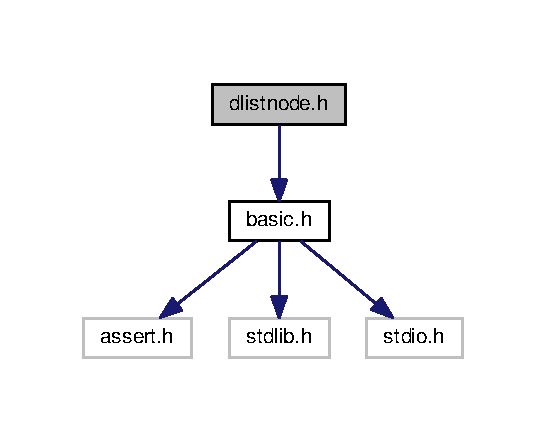
\includegraphics[width=262pt]{dlistnode_8h__incl}
\end{center}
\end{figure}
This graph shows which files directly or indirectly include this file\+:
\nopagebreak
\begin{figure}[H]
\begin{center}
\leavevmode
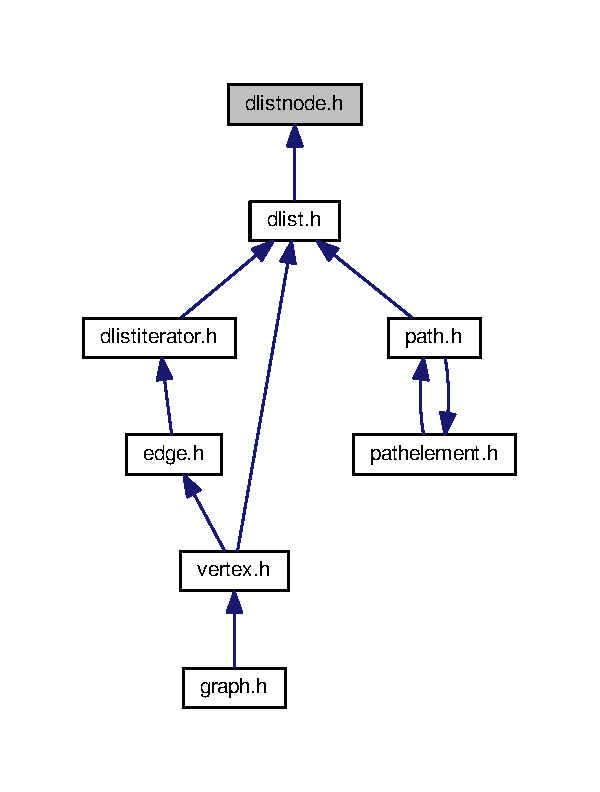
\includegraphics[width=288pt]{dlistnode_8h__dep__incl}
\end{center}
\end{figure}
\subsection*{Data Structures}
\begin{DoxyCompactItemize}
\item 
struct \hyperlink{structDListNode}{D\+List\+Node}
\begin{DoxyCompactList}\small\item\em The atomic data structure of a generic doubly linked list. (\hyperlink{structDList}{D\+List}) \end{DoxyCompactList}\end{DoxyCompactItemize}
\subsection*{Typedefs}
\begin{DoxyCompactItemize}
\item 
typedef struct \hyperlink{structDListNode}{D\+List\+Node} {\bfseries D\+List\+Node}\hypertarget{dlistnode_8h_a04751e7d05a5785b4961ee93887cb620}{}\label{dlistnode_8h_a04751e7d05a5785b4961ee93887cb620}

\end{DoxyCompactItemize}
\subsection*{Functions}
\begin{DoxyCompactItemize}
\item 
\hyperlink{structDListNode}{D\+List\+Node} $\ast$ \hyperlink{dlistnode_8h_a2bb091387ca2ee7d29e887586be08baa}{d\+List\+Node\+\_\+new} (\hyperlink{basic_8h_a5f051eaa796886555205c751e6d530f4}{Data} data, \hyperlink{structDListNode}{D\+List\+Node} $\ast$prev, \hyperlink{structDListNode}{D\+List\+Node} $\ast$next)
\begin{DoxyCompactList}\small\item\em Allocates and initializes a node. \end{DoxyCompactList}\item 
void \hyperlink{dlistnode_8h_aead4167ba3baf692d5b816755f420b67}{d\+List\+Node\+\_\+destroy} (\hyperlink{structDListNode}{D\+List\+Node} $\ast$node)
\begin{DoxyCompactList}\small\item\em Frees the memory of the node. \end{DoxyCompactList}\end{DoxyCompactItemize}


\subsection{Detailed Description}
A node in a generic doubly linked list. 

\begin{DoxyAuthor}{Author}
Philipp Badenhoop 
\end{DoxyAuthor}
\begin{DoxyDate}{Date}
4 Jun 2016 
\end{DoxyDate}


\subsection{Function Documentation}
\index{dlistnode.\+h@{dlistnode.\+h}!d\+List\+Node\+\_\+destroy@{d\+List\+Node\+\_\+destroy}}
\index{d\+List\+Node\+\_\+destroy@{d\+List\+Node\+\_\+destroy}!dlistnode.\+h@{dlistnode.\+h}}
\subsubsection[{\texorpdfstring{d\+List\+Node\+\_\+destroy(\+D\+List\+Node $\ast$node)}{dListNode_destroy(DListNode *node)}}]{\setlength{\rightskip}{0pt plus 5cm}void d\+List\+Node\+\_\+destroy (
\begin{DoxyParamCaption}
\item[{{\bf D\+List\+Node} $\ast$}]{node}
\end{DoxyParamCaption}
)}\hypertarget{dlistnode_8h_aead4167ba3baf692d5b816755f420b67}{}\label{dlistnode_8h_aead4167ba3baf692d5b816755f420b67}


Frees the memory of the node. 


\begin{DoxyParams}{Parameters}
{\em node} & The node to be destroyed. \\
\hline
\end{DoxyParams}
\index{dlistnode.\+h@{dlistnode.\+h}!d\+List\+Node\+\_\+new@{d\+List\+Node\+\_\+new}}
\index{d\+List\+Node\+\_\+new@{d\+List\+Node\+\_\+new}!dlistnode.\+h@{dlistnode.\+h}}
\subsubsection[{\texorpdfstring{d\+List\+Node\+\_\+new(\+Data data, D\+List\+Node $\ast$prev, D\+List\+Node $\ast$next)}{dListNode_new(Data data, DListNode *prev, DListNode *next)}}]{\setlength{\rightskip}{0pt plus 5cm}{\bf D\+List\+Node}$\ast$ d\+List\+Node\+\_\+new (
\begin{DoxyParamCaption}
\item[{{\bf Data}}]{data, }
\item[{{\bf D\+List\+Node} $\ast$}]{prev, }
\item[{{\bf D\+List\+Node} $\ast$}]{next}
\end{DoxyParamCaption}
)}\hypertarget{dlistnode_8h_a2bb091387ca2ee7d29e887586be08baa}{}\label{dlistnode_8h_a2bb091387ca2ee7d29e887586be08baa}


Allocates and initializes a node. 


\begin{DoxyParams}{Parameters}
{\em data} & The generic data the node stores. \\
\hline
{\em prev} & The previous node. \\
\hline
{\em next} & The next node. \\
\hline
\end{DoxyParams}
\begin{DoxyReturn}{Returns}
A pointer to the created node. 
\end{DoxyReturn}

\hypertarget{edge_8h}{}\section{edge.\+h File Reference}
\label{edge_8h}\index{edge.\+h@{edge.\+h}}


The edge between vertices in a graph.  


{\ttfamily \#include \char`\"{}basic.\+h\char`\"{}}\\*
{\ttfamily \#include \char`\"{}dlistiterator.\+h\char`\"{}}\\*
Include dependency graph for edge.\+h\+:\nopagebreak
\begin{figure}[H]
\begin{center}
\leavevmode
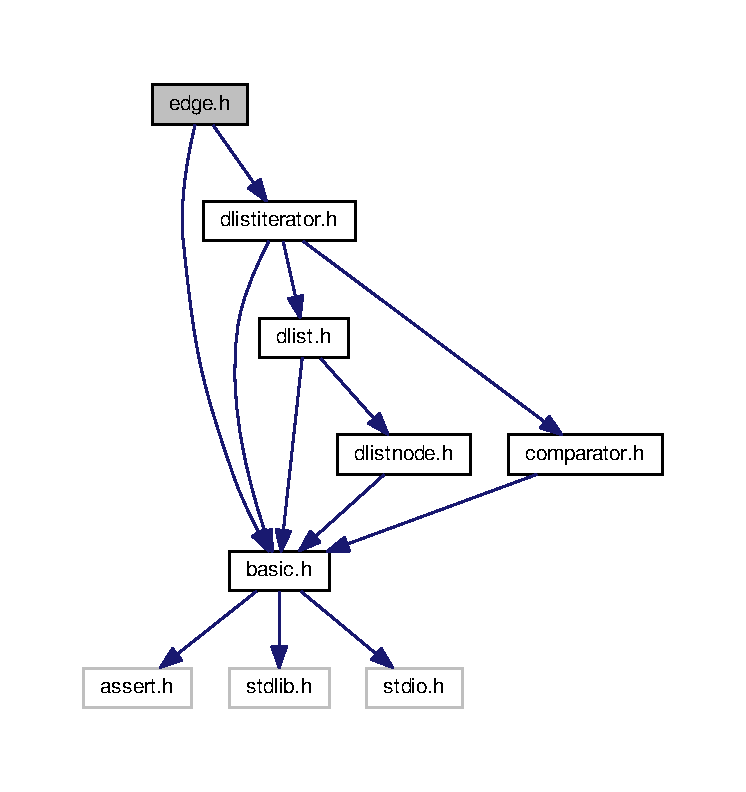
\includegraphics[width=350pt]{edge_8h__incl}
\end{center}
\end{figure}
This graph shows which files directly or indirectly include this file\+:\nopagebreak
\begin{figure}[H]
\begin{center}
\leavevmode
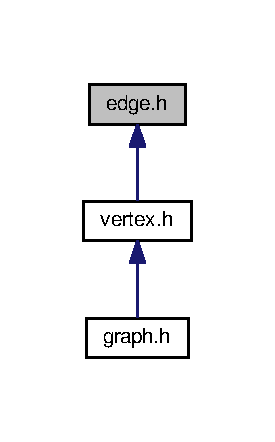
\includegraphics[width=132pt]{edge_8h__dep__incl}
\end{center}
\end{figure}
\subsection*{Data Structures}
\begin{DoxyCompactItemize}
\item 
struct \hyperlink{structEdge}{Edge}
\end{DoxyCompactItemize}
\subsection*{Typedefs}
\begin{DoxyCompactItemize}
\item 
typedef struct \hyperlink{structEdge}{Edge} \hyperlink{edge_8h_a89b91ff6921535d9c8215110f215c2c7}{Edge}\hypertarget{edge_8h_a89b91ff6921535d9c8215110f215c2c7}{}\label{edge_8h_a89b91ff6921535d9c8215110f215c2c7}

\begin{DoxyCompactList}\small\item\em The edge between vertices in a graph. Next to the vertex number of the vertex which it goes to, it also stores an iterator to find its corresponding edge, meaning the edge in a bidirectional graph. This is important because when we remove this edge, we must also remove the corresponding edge and we want that to happen fast! Using this approach, we don\textquotesingle{}t have to search it incrementally in a doubly linked list but rather destroy it immediately. \end{DoxyCompactList}\end{DoxyCompactItemize}
\subsection*{Functions}
\begin{DoxyCompactItemize}
\item 
\hyperlink{structEdge}{Edge} $\ast$ \hyperlink{edge_8h_a267730486ea8d66db4c084a5f1049e4a}{edge\+\_\+new} (int to\+Vertex\+Num)
\begin{DoxyCompactList}\small\item\em Allocates and initializes a new edge. \end{DoxyCompactList}\item 
void \hyperlink{edge_8h_ac1c4b5e7b84e8d9b6584345825145e0b}{edge\+\_\+destroy} (\hyperlink{structEdge}{Edge} $\ast$edge)
\begin{DoxyCompactList}\small\item\em Destroys the edge and its iterator to the corresponding edge. \end{DoxyCompactList}\item 
int \hyperlink{edge_8h_abc918fa1d6e6de0234fd1b6a4f4c0a04}{edge\+\_\+get\+To\+Vertex\+Num} (\hyperlink{structEdge}{Edge} $\ast$edge)
\item 
void \hyperlink{edge_8h_a4203862b7878eb9ccb5efa14ca1a4ab2}{edge\+\_\+set\+Corresponding\+Edge\+Iterator} (\hyperlink{structEdge}{Edge} $\ast$edge, \hyperlink{structDListIterator}{D\+List\+Iterator} $\ast$corresponding\+Edge\+Iterator)
\begin{DoxyCompactList}\small\item\em Sets the iterator to the corresponding edge. \end{DoxyCompactList}\item 
\hyperlink{structDListIterator}{D\+List\+Iterator} $\ast$ \hyperlink{edge_8h_af3313d551e1401e844a350d1c7a1d16c}{edge\+\_\+get\+Corresponding\+Edge\+Iterator} (\hyperlink{structEdge}{Edge} $\ast$edge)
\item 
bool \hyperlink{edge_8h_a4ad4b37d38fc5a32b98cf8d2f079f6aa}{edge\+\_\+equals} (\hyperlink{structEdge}{Edge} $\ast$edge1, \hyperlink{structEdge}{Edge} $\ast$edge2)
\begin{DoxyCompactList}\small\item\em Compares two edges. \end{DoxyCompactList}\end{DoxyCompactItemize}


\subsection{Detailed Description}
The edge between vertices in a graph. 

\begin{DoxyAuthor}{Author}
Philipp Badenhoop 
\end{DoxyAuthor}
\begin{DoxyDate}{Date}
6 Jun 2016 
\end{DoxyDate}


\subsection{Function Documentation}
\index{edge.\+h@{edge.\+h}!edge\+\_\+destroy@{edge\+\_\+destroy}}
\index{edge\+\_\+destroy@{edge\+\_\+destroy}!edge.\+h@{edge.\+h}}
\subsubsection[{\texorpdfstring{edge\+\_\+destroy(\+Edge $\ast$edge)}{edge_destroy(Edge *edge)}}]{\setlength{\rightskip}{0pt plus 5cm}void edge\+\_\+destroy (
\begin{DoxyParamCaption}
\item[{{\bf Edge} $\ast$}]{edge}
\end{DoxyParamCaption}
)}\hypertarget{edge_8h_ac1c4b5e7b84e8d9b6584345825145e0b}{}\label{edge_8h_ac1c4b5e7b84e8d9b6584345825145e0b}


Destroys the edge and its iterator to the corresponding edge. 


\begin{DoxyParams}{Parameters}
{\em edge} & \\
\hline
\end{DoxyParams}
\index{edge.\+h@{edge.\+h}!edge\+\_\+equals@{edge\+\_\+equals}}
\index{edge\+\_\+equals@{edge\+\_\+equals}!edge.\+h@{edge.\+h}}
\subsubsection[{\texorpdfstring{edge\+\_\+equals(\+Edge $\ast$edge1, Edge $\ast$edge2)}{edge_equals(Edge *edge1, Edge *edge2)}}]{\setlength{\rightskip}{0pt plus 5cm}bool edge\+\_\+equals (
\begin{DoxyParamCaption}
\item[{{\bf Edge} $\ast$}]{edge1, }
\item[{{\bf Edge} $\ast$}]{edge2}
\end{DoxyParamCaption}
)}\hypertarget{edge_8h_a4ad4b37d38fc5a32b98cf8d2f079f6aa}{}\label{edge_8h_a4ad4b37d38fc5a32b98cf8d2f079f6aa}


Compares two edges. 


\begin{DoxyParams}{Parameters}
{\em edge1} & \\
\hline
{\em edge2} & \\
\hline
\end{DoxyParams}
\begin{DoxyReturn}{Returns}
true, if the vertex number the edges go to are equal. 
\end{DoxyReturn}
\index{edge.\+h@{edge.\+h}!edge\+\_\+get\+Corresponding\+Edge\+Iterator@{edge\+\_\+get\+Corresponding\+Edge\+Iterator}}
\index{edge\+\_\+get\+Corresponding\+Edge\+Iterator@{edge\+\_\+get\+Corresponding\+Edge\+Iterator}!edge.\+h@{edge.\+h}}
\subsubsection[{\texorpdfstring{edge\+\_\+get\+Corresponding\+Edge\+Iterator(\+Edge $\ast$edge)}{edge_getCorrespondingEdgeIterator(Edge *edge)}}]{\setlength{\rightskip}{0pt plus 5cm}{\bf D\+List\+Iterator}$\ast$ edge\+\_\+get\+Corresponding\+Edge\+Iterator (
\begin{DoxyParamCaption}
\item[{{\bf Edge} $\ast$}]{edge}
\end{DoxyParamCaption}
)}\hypertarget{edge_8h_af3313d551e1401e844a350d1c7a1d16c}{}\label{edge_8h_af3313d551e1401e844a350d1c7a1d16c}

\begin{DoxyParams}{Parameters}
{\em edge} & \\
\hline
\end{DoxyParams}
\begin{DoxyReturn}{Returns}
Gets the iterator to teh corresponding edge. 
\end{DoxyReturn}
\index{edge.\+h@{edge.\+h}!edge\+\_\+get\+To\+Vertex\+Num@{edge\+\_\+get\+To\+Vertex\+Num}}
\index{edge\+\_\+get\+To\+Vertex\+Num@{edge\+\_\+get\+To\+Vertex\+Num}!edge.\+h@{edge.\+h}}
\subsubsection[{\texorpdfstring{edge\+\_\+get\+To\+Vertex\+Num(\+Edge $\ast$edge)}{edge_getToVertexNum(Edge *edge)}}]{\setlength{\rightskip}{0pt plus 5cm}int edge\+\_\+get\+To\+Vertex\+Num (
\begin{DoxyParamCaption}
\item[{{\bf Edge} $\ast$}]{edge}
\end{DoxyParamCaption}
)}\hypertarget{edge_8h_abc918fa1d6e6de0234fd1b6a4f4c0a04}{}\label{edge_8h_abc918fa1d6e6de0234fd1b6a4f4c0a04}

\begin{DoxyParams}{Parameters}
{\em edge} & \\
\hline
\end{DoxyParams}
\begin{DoxyReturn}{Returns}
The vertex number this edge goes to. 
\end{DoxyReturn}
\index{edge.\+h@{edge.\+h}!edge\+\_\+new@{edge\+\_\+new}}
\index{edge\+\_\+new@{edge\+\_\+new}!edge.\+h@{edge.\+h}}
\subsubsection[{\texorpdfstring{edge\+\_\+new(int to\+Vertex\+Num)}{edge_new(int toVertexNum)}}]{\setlength{\rightskip}{0pt plus 5cm}{\bf Edge}$\ast$ edge\+\_\+new (
\begin{DoxyParamCaption}
\item[{int}]{to\+Vertex\+Num}
\end{DoxyParamCaption}
)}\hypertarget{edge_8h_a267730486ea8d66db4c084a5f1049e4a}{}\label{edge_8h_a267730486ea8d66db4c084a5f1049e4a}


Allocates and initializes a new edge. 


\begin{DoxyParams}{Parameters}
{\em to\+Vertex\+Num} & \\
\hline
\end{DoxyParams}
\begin{DoxyReturn}{Returns}
The pointer to the new edge. 
\end{DoxyReturn}
\index{edge.\+h@{edge.\+h}!edge\+\_\+set\+Corresponding\+Edge\+Iterator@{edge\+\_\+set\+Corresponding\+Edge\+Iterator}}
\index{edge\+\_\+set\+Corresponding\+Edge\+Iterator@{edge\+\_\+set\+Corresponding\+Edge\+Iterator}!edge.\+h@{edge.\+h}}
\subsubsection[{\texorpdfstring{edge\+\_\+set\+Corresponding\+Edge\+Iterator(\+Edge $\ast$edge, D\+List\+Iterator $\ast$corresponding\+Edge\+Iterator)}{edge_setCorrespondingEdgeIterator(Edge *edge, DListIterator *correspondingEdgeIterator)}}]{\setlength{\rightskip}{0pt plus 5cm}void edge\+\_\+set\+Corresponding\+Edge\+Iterator (
\begin{DoxyParamCaption}
\item[{{\bf Edge} $\ast$}]{edge, }
\item[{{\bf D\+List\+Iterator} $\ast$}]{corresponding\+Edge\+Iterator}
\end{DoxyParamCaption}
)}\hypertarget{edge_8h_a4203862b7878eb9ccb5efa14ca1a4ab2}{}\label{edge_8h_a4203862b7878eb9ccb5efa14ca1a4ab2}


Sets the iterator to the corresponding edge. 


\begin{DoxyParams}{Parameters}
{\em edge} & \\
\hline
{\em corresponding\+Edge\+Iterator} & \\
\hline
\end{DoxyParams}

\hypertarget{graph_8h}{}\section{graph.\+h File Reference}
\label{graph_8h}\index{graph.\+h@{graph.\+h}}


A graph containing vertices which are connected through edges.  


{\ttfamily \#include \char`\"{}basic.\+h\char`\"{}}\\*
{\ttfamily \#include \char`\"{}vertex.\+h\char`\"{}}\\*
Include dependency graph for graph.\+h\+:\nopagebreak
\begin{figure}[H]
\begin{center}
\leavevmode
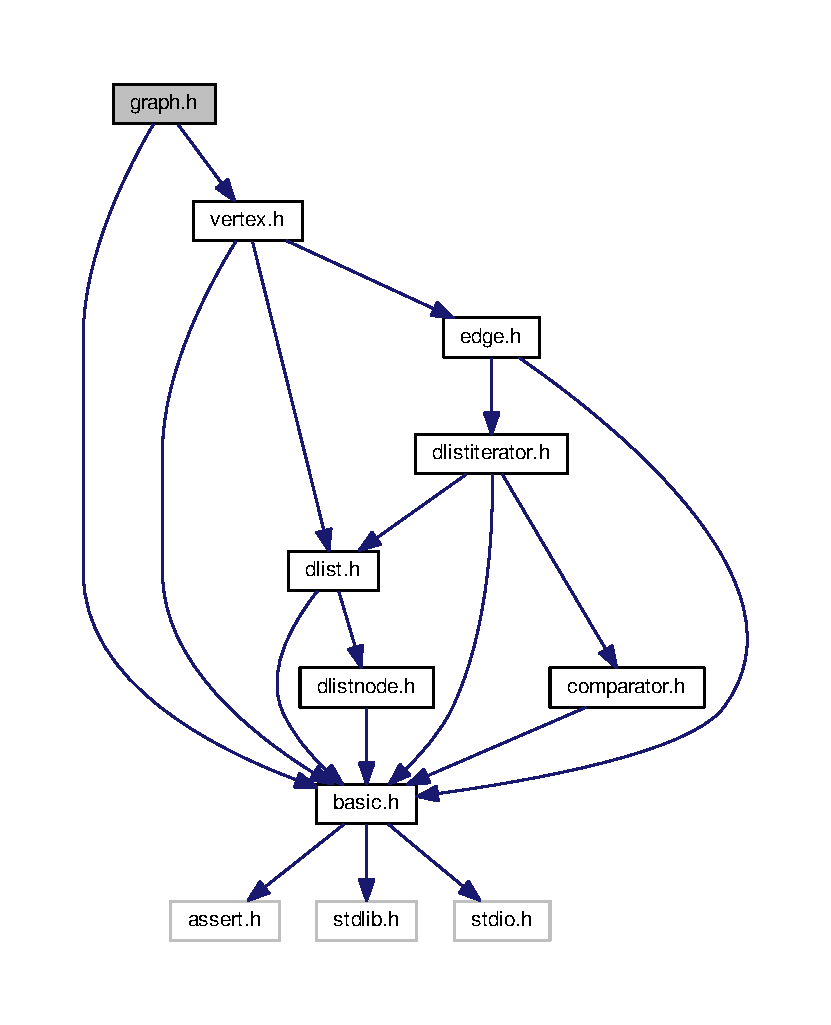
\includegraphics[width=350pt]{graph_8h__incl}
\end{center}
\end{figure}
\subsection*{Data Structures}
\begin{DoxyCompactItemize}
\item 
struct \hyperlink{structGraph}{Graph}
\end{DoxyCompactItemize}
\subsection*{Functions}
\begin{DoxyCompactItemize}
\item 
\hyperlink{structGraph}{Graph} $\ast$ \hyperlink{graph_8h_a75a12b58b016fe46a877a2ed05a39e92}{graph\+\_\+new} (int vertex\+Count)
\begin{DoxyCompactList}\small\item\em Allocates and initializes a new graph. \end{DoxyCompactList}\item 
void \hyperlink{graph_8h_a0587b1cdbfee591e41793bef7f8e0c87}{graph\+\_\+destroy} (\hyperlink{structGraph}{Graph} $\ast$graph)
\begin{DoxyCompactList}\small\item\em Simply frees the poiner to the graph. \end{DoxyCompactList}\item 
void \hyperlink{graph_8h_ae1009ab159ee614b8ec548f328642f01}{graph\+\_\+destroy\+All} (\hyperlink{structGraph}{Graph} $\ast$graph)
\begin{DoxyCompactList}\small\item\em Frees the pointer to the graph and completely destroys the structure of the graph including all vertices and their edges. \end{DoxyCompactList}\item 
void \hyperlink{graph_8h_a5f8f8fae3e276ddab6c7c475e5e1661a}{graph\+\_\+set\+Vertex} (\hyperlink{structGraph}{Graph} $\ast$graph, \hyperlink{structVertex}{Vertex} $\ast$vertex, int vertex\+Num)
\item 
\hyperlink{structVertex}{Vertex} $\ast$ \hyperlink{graph_8h_afdf769b4c7574785c309eec2c7cbe723}{graph\+\_\+get\+Vertex} (\hyperlink{structGraph}{Graph} $\ast$graph, int vertex\+Num)
\item 
int \hyperlink{graph_8h_af7058e7d1bb728f0758541a70c80733f}{graph\+\_\+get\+Vertex\+Count} (\hyperlink{structGraph}{Graph} $\ast$graph)
\item 
void \hyperlink{graph_8h_a371dd1edd6d8e3559d773563ee82ca2b}{graph\+\_\+add\+Vertex} (\hyperlink{structGraph}{Graph} $\ast$graph)
\begin{DoxyCompactList}\small\item\em This adds a vertex to the graph. \end{DoxyCompactList}\item 
void \hyperlink{graph_8h_a2c7624028cfd0b4c60f4acfdbc9198b7}{graph\+\_\+add\+Edge\+Pair} (\hyperlink{structGraph}{Graph} $\ast$graph, int vertex\+Num1, int vertex\+Num2)
\begin{DoxyCompactList}\small\item\em Adds a bidirectional edge betweenn two vertices. \end{DoxyCompactList}\item 
bool \hyperlink{graph_8h_ac2804aa4086deb2e949c900985361284}{graph\+\_\+remove\+Edge\+Pair} (\hyperlink{structGraph}{Graph} $\ast$graph, int vertex\+Num1, int vertex\+Num2)
\begin{DoxyCompactList}\small\item\em Removes a bidirectional edge between two vertices. \end{DoxyCompactList}\item 
bool \hyperlink{graph_8h_a19ee4af3118fbcb1e5874fed6ca3ac29}{graph\+\_\+has\+Edges} (\hyperlink{structGraph}{Graph} $\ast$graph)
\end{DoxyCompactItemize}


\subsection{Detailed Description}
A graph containing vertices which are connected through edges. 

\begin{DoxyAuthor}{Author}
Philipp Badenhoop 
\end{DoxyAuthor}
\begin{DoxyDate}{Date}
6 Jun 2016 
\end{DoxyDate}


\subsection{Function Documentation}
\index{graph.\+h@{graph.\+h}!graph\+\_\+add\+Edge\+Pair@{graph\+\_\+add\+Edge\+Pair}}
\index{graph\+\_\+add\+Edge\+Pair@{graph\+\_\+add\+Edge\+Pair}!graph.\+h@{graph.\+h}}
\subsubsection[{\texorpdfstring{graph\+\_\+add\+Edge\+Pair(\+Graph $\ast$graph, int vertex\+Num1, int vertex\+Num2)}{graph_addEdgePair(Graph *graph, int vertexNum1, int vertexNum2)}}]{\setlength{\rightskip}{0pt plus 5cm}void graph\+\_\+add\+Edge\+Pair (
\begin{DoxyParamCaption}
\item[{{\bf Graph} $\ast$}]{graph, }
\item[{int}]{vertex\+Num1, }
\item[{int}]{vertex\+Num2}
\end{DoxyParamCaption}
)}\hypertarget{graph_8h_a2c7624028cfd0b4c60f4acfdbc9198b7}{}\label{graph_8h_a2c7624028cfd0b4c60f4acfdbc9198b7}


Adds a bidirectional edge betweenn two vertices. 


\begin{DoxyParams}{Parameters}
{\em graph} & \\
\hline
{\em vertex\+Num1} & \\
\hline
{\em vertex\+Num2} & \\
\hline
\end{DoxyParams}
\index{graph.\+h@{graph.\+h}!graph\+\_\+add\+Vertex@{graph\+\_\+add\+Vertex}}
\index{graph\+\_\+add\+Vertex@{graph\+\_\+add\+Vertex}!graph.\+h@{graph.\+h}}
\subsubsection[{\texorpdfstring{graph\+\_\+add\+Vertex(\+Graph $\ast$graph)}{graph_addVertex(Graph *graph)}}]{\setlength{\rightskip}{0pt plus 5cm}void graph\+\_\+add\+Vertex (
\begin{DoxyParamCaption}
\item[{{\bf Graph} $\ast$}]{graph}
\end{DoxyParamCaption}
)}\hypertarget{graph_8h_a371dd1edd6d8e3559d773563ee82ca2b}{}\label{graph_8h_a371dd1edd6d8e3559d773563ee82ca2b}


This adds a vertex to the graph. 


\begin{DoxyParams}{Parameters}
{\em graph} & \\
\hline
\end{DoxyParams}
\begin{DoxyAttention}{Attention}
This function can be slow on a graph with a large number of vertices since it creates a new array of the current size + 1 and copies all vertices from the old array into the new one. 
\end{DoxyAttention}
\index{graph.\+h@{graph.\+h}!graph\+\_\+destroy@{graph\+\_\+destroy}}
\index{graph\+\_\+destroy@{graph\+\_\+destroy}!graph.\+h@{graph.\+h}}
\subsubsection[{\texorpdfstring{graph\+\_\+destroy(\+Graph $\ast$graph)}{graph_destroy(Graph *graph)}}]{\setlength{\rightskip}{0pt plus 5cm}void graph\+\_\+destroy (
\begin{DoxyParamCaption}
\item[{{\bf Graph} $\ast$}]{graph}
\end{DoxyParamCaption}
)}\hypertarget{graph_8h_a0587b1cdbfee591e41793bef7f8e0c87}{}\label{graph_8h_a0587b1cdbfee591e41793bef7f8e0c87}


Simply frees the poiner to the graph. 


\begin{DoxyParams}{Parameters}
{\em graph} & \\
\hline
\end{DoxyParams}
\index{graph.\+h@{graph.\+h}!graph\+\_\+destroy\+All@{graph\+\_\+destroy\+All}}
\index{graph\+\_\+destroy\+All@{graph\+\_\+destroy\+All}!graph.\+h@{graph.\+h}}
\subsubsection[{\texorpdfstring{graph\+\_\+destroy\+All(\+Graph $\ast$graph)}{graph_destroyAll(Graph *graph)}}]{\setlength{\rightskip}{0pt plus 5cm}void graph\+\_\+destroy\+All (
\begin{DoxyParamCaption}
\item[{{\bf Graph} $\ast$}]{graph}
\end{DoxyParamCaption}
)}\hypertarget{graph_8h_ae1009ab159ee614b8ec548f328642f01}{}\label{graph_8h_ae1009ab159ee614b8ec548f328642f01}


Frees the pointer to the graph and completely destroys the structure of the graph including all vertices and their edges. 


\begin{DoxyParams}{Parameters}
{\em graph} & \\
\hline
\end{DoxyParams}
\index{graph.\+h@{graph.\+h}!graph\+\_\+get\+Vertex@{graph\+\_\+get\+Vertex}}
\index{graph\+\_\+get\+Vertex@{graph\+\_\+get\+Vertex}!graph.\+h@{graph.\+h}}
\subsubsection[{\texorpdfstring{graph\+\_\+get\+Vertex(\+Graph $\ast$graph, int vertex\+Num)}{graph_getVertex(Graph *graph, int vertexNum)}}]{\setlength{\rightskip}{0pt plus 5cm}{\bf Vertex}$\ast$ graph\+\_\+get\+Vertex (
\begin{DoxyParamCaption}
\item[{{\bf Graph} $\ast$}]{graph, }
\item[{int}]{vertex\+Num}
\end{DoxyParamCaption}
)}\hypertarget{graph_8h_afdf769b4c7574785c309eec2c7cbe723}{}\label{graph_8h_afdf769b4c7574785c309eec2c7cbe723}

\begin{DoxyParams}{Parameters}
{\em graph} & \\
\hline
{\em vertex\+Num} & \\
\hline
\end{DoxyParams}
\begin{DoxyReturn}{Returns}
Get the vertex object at a specified vertex number. 
\end{DoxyReturn}
\index{graph.\+h@{graph.\+h}!graph\+\_\+get\+Vertex\+Count@{graph\+\_\+get\+Vertex\+Count}}
\index{graph\+\_\+get\+Vertex\+Count@{graph\+\_\+get\+Vertex\+Count}!graph.\+h@{graph.\+h}}
\subsubsection[{\texorpdfstring{graph\+\_\+get\+Vertex\+Count(\+Graph $\ast$graph)}{graph_getVertexCount(Graph *graph)}}]{\setlength{\rightskip}{0pt plus 5cm}int graph\+\_\+get\+Vertex\+Count (
\begin{DoxyParamCaption}
\item[{{\bf Graph} $\ast$}]{graph}
\end{DoxyParamCaption}
)}\hypertarget{graph_8h_af7058e7d1bb728f0758541a70c80733f}{}\label{graph_8h_af7058e7d1bb728f0758541a70c80733f}

\begin{DoxyParams}{Parameters}
{\em graph} & \\
\hline
\end{DoxyParams}
\begin{DoxyReturn}{Returns}
The number of vertices in the graph. 
\end{DoxyReturn}
\index{graph.\+h@{graph.\+h}!graph\+\_\+has\+Edges@{graph\+\_\+has\+Edges}}
\index{graph\+\_\+has\+Edges@{graph\+\_\+has\+Edges}!graph.\+h@{graph.\+h}}
\subsubsection[{\texorpdfstring{graph\+\_\+has\+Edges(\+Graph $\ast$graph)}{graph_hasEdges(Graph *graph)}}]{\setlength{\rightskip}{0pt plus 5cm}bool graph\+\_\+has\+Edges (
\begin{DoxyParamCaption}
\item[{{\bf Graph} $\ast$}]{graph}
\end{DoxyParamCaption}
)}\hypertarget{graph_8h_a19ee4af3118fbcb1e5874fed6ca3ac29}{}\label{graph_8h_a19ee4af3118fbcb1e5874fed6ca3ac29}

\begin{DoxyParams}{Parameters}
{\em graph} & \\
\hline
\end{DoxyParams}
\begin{DoxyReturn}{Returns}
true, if there is at least one vertex with an edge to another vertex. 
\end{DoxyReturn}
\index{graph.\+h@{graph.\+h}!graph\+\_\+new@{graph\+\_\+new}}
\index{graph\+\_\+new@{graph\+\_\+new}!graph.\+h@{graph.\+h}}
\subsubsection[{\texorpdfstring{graph\+\_\+new(int vertex\+Count)}{graph_new(int vertexCount)}}]{\setlength{\rightskip}{0pt plus 5cm}{\bf Graph}$\ast$ graph\+\_\+new (
\begin{DoxyParamCaption}
\item[{int}]{vertex\+Count}
\end{DoxyParamCaption}
)}\hypertarget{graph_8h_a75a12b58b016fe46a877a2ed05a39e92}{}\label{graph_8h_a75a12b58b016fe46a877a2ed05a39e92}


Allocates and initializes a new graph. 


\begin{DoxyParams}{Parameters}
{\em vertex\+Count} & \\
\hline
\end{DoxyParams}
\begin{DoxyReturn}{Returns}
The pointer to the new graph. 
\end{DoxyReturn}
\index{graph.\+h@{graph.\+h}!graph\+\_\+remove\+Edge\+Pair@{graph\+\_\+remove\+Edge\+Pair}}
\index{graph\+\_\+remove\+Edge\+Pair@{graph\+\_\+remove\+Edge\+Pair}!graph.\+h@{graph.\+h}}
\subsubsection[{\texorpdfstring{graph\+\_\+remove\+Edge\+Pair(\+Graph $\ast$graph, int vertex\+Num1, int vertex\+Num2)}{graph_removeEdgePair(Graph *graph, int vertexNum1, int vertexNum2)}}]{\setlength{\rightskip}{0pt plus 5cm}bool graph\+\_\+remove\+Edge\+Pair (
\begin{DoxyParamCaption}
\item[{{\bf Graph} $\ast$}]{graph, }
\item[{int}]{vertex\+Num1, }
\item[{int}]{vertex\+Num2}
\end{DoxyParamCaption}
)}\hypertarget{graph_8h_ac2804aa4086deb2e949c900985361284}{}\label{graph_8h_ac2804aa4086deb2e949c900985361284}


Removes a bidirectional edge between two vertices. 


\begin{DoxyParams}{Parameters}
{\em graph} & \\
\hline
{\em vertex\+Num1} & \\
\hline
{\em vertex\+Num2} & \\
\hline
\end{DoxyParams}
\begin{DoxyReturn}{Returns}
true, if the given edge was found and removed, else false. 
\end{DoxyReturn}
\index{graph.\+h@{graph.\+h}!graph\+\_\+set\+Vertex@{graph\+\_\+set\+Vertex}}
\index{graph\+\_\+set\+Vertex@{graph\+\_\+set\+Vertex}!graph.\+h@{graph.\+h}}
\subsubsection[{\texorpdfstring{graph\+\_\+set\+Vertex(\+Graph $\ast$graph, Vertex $\ast$vertex, int vertex\+Num)}{graph_setVertex(Graph *graph, Vertex *vertex, int vertexNum)}}]{\setlength{\rightskip}{0pt plus 5cm}void graph\+\_\+set\+Vertex (
\begin{DoxyParamCaption}
\item[{{\bf Graph} $\ast$}]{graph, }
\item[{{\bf Vertex} $\ast$}]{vertex, }
\item[{int}]{vertex\+Num}
\end{DoxyParamCaption}
)}\hypertarget{graph_8h_a5f8f8fae3e276ddab6c7c475e5e1661a}{}\label{graph_8h_a5f8f8fae3e276ddab6c7c475e5e1661a}

\begin{DoxyParams}{Parameters}
{\em graph} & \\
\hline
{\em vertex} & \\
\hline
{\em vertex\+Num} & \\
\hline
\end{DoxyParams}

\hypertarget{path_8h}{}\section{path.\+h File Reference}
\label{path_8h}\index{path.\+h@{path.\+h}}


A path of vertices of a graph.  


{\ttfamily \#include \char`\"{}basic.\+h\char`\"{}}\\*
{\ttfamily \#include \char`\"{}dlist.\+h\char`\"{}}\\*
{\ttfamily \#include \char`\"{}pathelement.\+h\char`\"{}}\\*
Include dependency graph for path.\+h\+:
\nopagebreak
\begin{figure}[H]
\begin{center}
\leavevmode
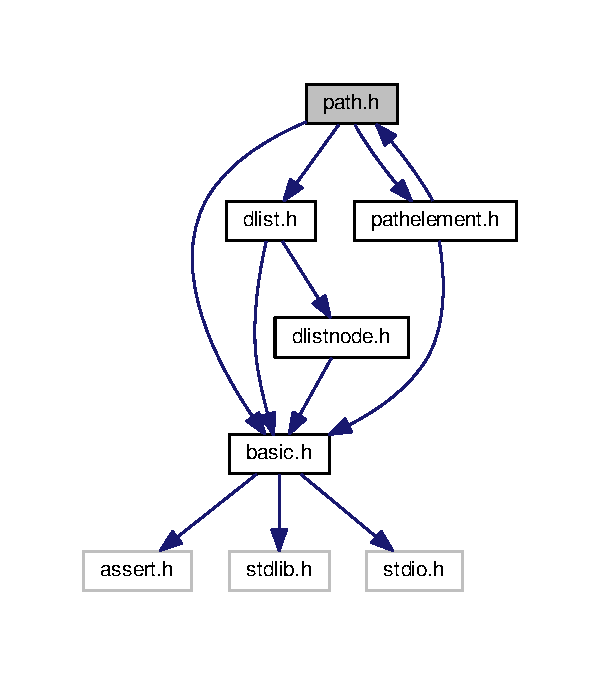
\includegraphics[width=288pt]{path_8h__incl}
\end{center}
\end{figure}
This graph shows which files directly or indirectly include this file\+:
\nopagebreak
\begin{figure}[H]
\begin{center}
\leavevmode
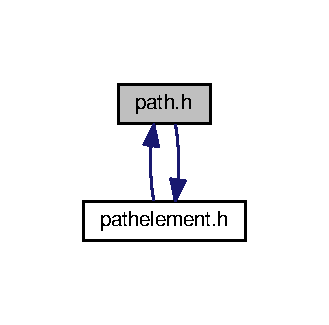
\includegraphics[width=158pt]{path_8h__dep__incl}
\end{center}
\end{figure}
\subsection*{Data Structures}
\begin{DoxyCompactItemize}
\item 
struct \hyperlink{structPath}{Path}
\begin{DoxyCompactList}\small\item\em This is just a container for a list of path elements which simply represent the vertices. \end{DoxyCompactList}\end{DoxyCompactItemize}
\subsection*{Functions}
\begin{DoxyCompactItemize}
\item 
\hyperlink{structPath}{Path} $\ast$ \hyperlink{path_8h_a9efa22a6ca425df4d58e6f20d370a410}{path\+\_\+new} (void)
\begin{DoxyCompactList}\small\item\em Allocates and initializes the path. \end{DoxyCompactList}\item 
void \hyperlink{path_8h_a5fb84b0cb40746e2e75ea95ccbc4117b}{path\+\_\+destroy} (\hyperlink{structPath}{Path} $\ast$path)
\begin{DoxyCompactList}\small\item\em Simply frees the pointer to the path. \end{DoxyCompactList}\item 
void \hyperlink{path_8h_ac30e783c45a72ea7a9f6017ea9dac7d4}{path\+\_\+destroy\+All} (\hyperlink{structPath}{Path} $\ast$path)
\begin{DoxyCompactList}\small\item\em Frees the pointer to the path and destroys all its elements too. \end{DoxyCompactList}\item 
\hyperlink{structDList}{D\+List} $\ast$ \hyperlink{path_8h_abee4e0e79dc921ed0777ce51a8e218e2}{path\+\_\+get\+Elements} (\hyperlink{structPath}{Path} $\ast$path)
\item 
void \hyperlink{path_8h_ae60832c5f4528ee713445bd939cdb18c}{path\+\_\+append} (\hyperlink{structPath}{Path} $\ast$path, int vertex\+Num)
\begin{DoxyCompactList}\small\item\em Appends a path element with the specified vertex number to the path. \end{DoxyCompactList}\end{DoxyCompactItemize}


\subsection{Detailed Description}
A path of vertices of a graph. 

\begin{DoxyAuthor}{Author}
Philipp Badenhoop 
\end{DoxyAuthor}
\begin{DoxyDate}{Date}
6 Jun 2016 
\end{DoxyDate}


\subsection{Function Documentation}
\index{path.\+h@{path.\+h}!path\+\_\+append@{path\+\_\+append}}
\index{path\+\_\+append@{path\+\_\+append}!path.\+h@{path.\+h}}
\subsubsection[{\texorpdfstring{path\+\_\+append(\+Path $\ast$path, int vertex\+Num)}{path_append(Path *path, int vertexNum)}}]{\setlength{\rightskip}{0pt plus 5cm}void path\+\_\+append (
\begin{DoxyParamCaption}
\item[{{\bf Path} $\ast$}]{path, }
\item[{int}]{vertex\+Num}
\end{DoxyParamCaption}
)}\hypertarget{path_8h_ae60832c5f4528ee713445bd939cdb18c}{}\label{path_8h_ae60832c5f4528ee713445bd939cdb18c}


Appends a path element with the specified vertex number to the path. 


\begin{DoxyParams}{Parameters}
{\em path} & \\
\hline
{\em vertex\+Num} & \\
\hline
\end{DoxyParams}
\index{path.\+h@{path.\+h}!path\+\_\+destroy@{path\+\_\+destroy}}
\index{path\+\_\+destroy@{path\+\_\+destroy}!path.\+h@{path.\+h}}
\subsubsection[{\texorpdfstring{path\+\_\+destroy(\+Path $\ast$path)}{path_destroy(Path *path)}}]{\setlength{\rightskip}{0pt plus 5cm}void path\+\_\+destroy (
\begin{DoxyParamCaption}
\item[{{\bf Path} $\ast$}]{path}
\end{DoxyParamCaption}
)}\hypertarget{path_8h_a5fb84b0cb40746e2e75ea95ccbc4117b}{}\label{path_8h_a5fb84b0cb40746e2e75ea95ccbc4117b}


Simply frees the pointer to the path. 


\begin{DoxyParams}{Parameters}
{\em path} & \\
\hline
\end{DoxyParams}
\index{path.\+h@{path.\+h}!path\+\_\+destroy\+All@{path\+\_\+destroy\+All}}
\index{path\+\_\+destroy\+All@{path\+\_\+destroy\+All}!path.\+h@{path.\+h}}
\subsubsection[{\texorpdfstring{path\+\_\+destroy\+All(\+Path $\ast$path)}{path_destroyAll(Path *path)}}]{\setlength{\rightskip}{0pt plus 5cm}void path\+\_\+destroy\+All (
\begin{DoxyParamCaption}
\item[{{\bf Path} $\ast$}]{path}
\end{DoxyParamCaption}
)}\hypertarget{path_8h_ac30e783c45a72ea7a9f6017ea9dac7d4}{}\label{path_8h_ac30e783c45a72ea7a9f6017ea9dac7d4}


Frees the pointer to the path and destroys all its elements too. 


\begin{DoxyParams}{Parameters}
{\em path} & \\
\hline
\end{DoxyParams}
\index{path.\+h@{path.\+h}!path\+\_\+get\+Elements@{path\+\_\+get\+Elements}}
\index{path\+\_\+get\+Elements@{path\+\_\+get\+Elements}!path.\+h@{path.\+h}}
\subsubsection[{\texorpdfstring{path\+\_\+get\+Elements(\+Path $\ast$path)}{path_getElements(Path *path)}}]{\setlength{\rightskip}{0pt plus 5cm}{\bf D\+List}$\ast$ path\+\_\+get\+Elements (
\begin{DoxyParamCaption}
\item[{{\bf Path} $\ast$}]{path}
\end{DoxyParamCaption}
)}\hypertarget{path_8h_abee4e0e79dc921ed0777ce51a8e218e2}{}\label{path_8h_abee4e0e79dc921ed0777ce51a8e218e2}

\begin{DoxyParams}{Parameters}
{\em path} & \\
\hline
\end{DoxyParams}
\begin{DoxyReturn}{Returns}
The list of path elements. 
\end{DoxyReturn}
\index{path.\+h@{path.\+h}!path\+\_\+new@{path\+\_\+new}}
\index{path\+\_\+new@{path\+\_\+new}!path.\+h@{path.\+h}}
\subsubsection[{\texorpdfstring{path\+\_\+new(void)}{path_new(void)}}]{\setlength{\rightskip}{0pt plus 5cm}{\bf Path}$\ast$ path\+\_\+new (
\begin{DoxyParamCaption}
\item[{void}]{}
\end{DoxyParamCaption}
)}\hypertarget{path_8h_a9efa22a6ca425df4d58e6f20d370a410}{}\label{path_8h_a9efa22a6ca425df4d58e6f20d370a410}


Allocates and initializes the path. 

\begin{DoxyReturn}{Returns}
The pointer to the new path. 
\end{DoxyReturn}

\hypertarget{pathelement_8h}{}\section{pathelement.\+h File Reference}
\label{pathelement_8h}\index{pathelement.\+h@{pathelement.\+h}}


An element of a path of a graph.  


{\ttfamily \#include \char`\"{}basic.\+h\char`\"{}}\\*
{\ttfamily \#include \char`\"{}path.\+h\char`\"{}}\\*
Include dependency graph for pathelement.\+h\+:
\nopagebreak
\begin{figure}[H]
\begin{center}
\leavevmode
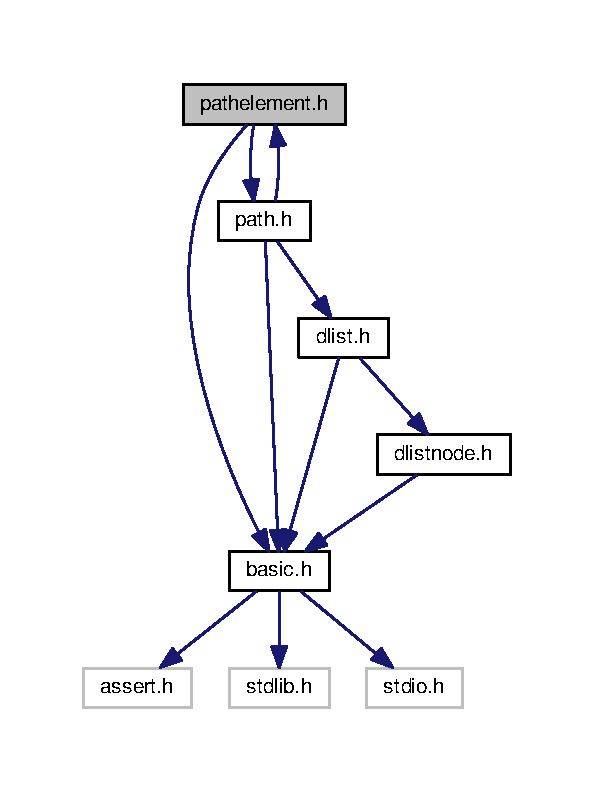
\includegraphics[width=285pt]{pathelement_8h__incl}
\end{center}
\end{figure}
This graph shows which files directly or indirectly include this file\+:
\nopagebreak
\begin{figure}[H]
\begin{center}
\leavevmode
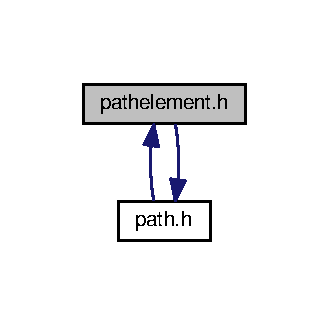
\includegraphics[width=158pt]{pathelement_8h__dep__incl}
\end{center}
\end{figure}
\subsection*{Data Structures}
\begin{DoxyCompactItemize}
\item 
struct \hyperlink{structPathElement}{Path\+Element}
\end{DoxyCompactItemize}
\subsection*{Functions}
\begin{DoxyCompactItemize}
\item 
\hyperlink{structPathElement}{Path\+Element} $\ast$ \hyperlink{pathelement_8h_a3a70b067c34a648f82ad4a96b622ab46}{path\+Element\+\_\+new} (int vertex\+Num)
\begin{DoxyCompactList}\small\item\em Allocates and initializes a new path element. \end{DoxyCompactList}\item 
void \hyperlink{pathelement_8h_a27bf0640d268c1054c162ab5ee4b1c0d}{path\+Element\+\_\+destroy} (\hyperlink{structPathElement}{Path\+Element} $\ast$element)
\begin{DoxyCompactList}\small\item\em Simply frees the pointer to the element. \end{DoxyCompactList}\item 
int \hyperlink{pathelement_8h_a44b34c29ea6ae65dbc61071015de03b1}{path\+Element\+\_\+get\+Vertex\+Num} (\hyperlink{structPathElement}{Path\+Element} $\ast$element)
\item 
bool \hyperlink{pathelement_8h_a4df5181d880f8cba07607039701ff45f}{path\+Element\+\_\+equals} (\hyperlink{structPathElement}{Path\+Element} $\ast$element1, \hyperlink{structPathElement}{Path\+Element} $\ast$element2)
\begin{DoxyCompactList}\small\item\em Compares two path elements. \end{DoxyCompactList}\end{DoxyCompactItemize}


\subsection{Detailed Description}
An element of a path of a graph. 

\begin{DoxyAuthor}{Author}
Philipp Badenhoop 
\end{DoxyAuthor}
\begin{DoxyDate}{Date}
6 Jun 2016 
\end{DoxyDate}


\subsection{Function Documentation}
\index{pathelement.\+h@{pathelement.\+h}!path\+Element\+\_\+destroy@{path\+Element\+\_\+destroy}}
\index{path\+Element\+\_\+destroy@{path\+Element\+\_\+destroy}!pathelement.\+h@{pathelement.\+h}}
\subsubsection[{\texorpdfstring{path\+Element\+\_\+destroy(\+Path\+Element $\ast$element)}{pathElement_destroy(PathElement *element)}}]{\setlength{\rightskip}{0pt plus 5cm}void path\+Element\+\_\+destroy (
\begin{DoxyParamCaption}
\item[{{\bf Path\+Element} $\ast$}]{element}
\end{DoxyParamCaption}
)}\hypertarget{pathelement_8h_a27bf0640d268c1054c162ab5ee4b1c0d}{}\label{pathelement_8h_a27bf0640d268c1054c162ab5ee4b1c0d}


Simply frees the pointer to the element. 


\begin{DoxyParams}{Parameters}
{\em element} & \\
\hline
\end{DoxyParams}
\index{pathelement.\+h@{pathelement.\+h}!path\+Element\+\_\+equals@{path\+Element\+\_\+equals}}
\index{path\+Element\+\_\+equals@{path\+Element\+\_\+equals}!pathelement.\+h@{pathelement.\+h}}
\subsubsection[{\texorpdfstring{path\+Element\+\_\+equals(\+Path\+Element $\ast$element1, Path\+Element $\ast$element2)}{pathElement_equals(PathElement *element1, PathElement *element2)}}]{\setlength{\rightskip}{0pt plus 5cm}bool path\+Element\+\_\+equals (
\begin{DoxyParamCaption}
\item[{{\bf Path\+Element} $\ast$}]{element1, }
\item[{{\bf Path\+Element} $\ast$}]{element2}
\end{DoxyParamCaption}
)}\hypertarget{pathelement_8h_a4df5181d880f8cba07607039701ff45f}{}\label{pathelement_8h_a4df5181d880f8cba07607039701ff45f}


Compares two path elements. 


\begin{DoxyParams}{Parameters}
{\em element1} & \\
\hline
{\em element2} & \\
\hline
\end{DoxyParams}
\begin{DoxyReturn}{Returns}
true, if the vertex number of the elements are equal. 
\end{DoxyReturn}
\index{pathelement.\+h@{pathelement.\+h}!path\+Element\+\_\+get\+Vertex\+Num@{path\+Element\+\_\+get\+Vertex\+Num}}
\index{path\+Element\+\_\+get\+Vertex\+Num@{path\+Element\+\_\+get\+Vertex\+Num}!pathelement.\+h@{pathelement.\+h}}
\subsubsection[{\texorpdfstring{path\+Element\+\_\+get\+Vertex\+Num(\+Path\+Element $\ast$element)}{pathElement_getVertexNum(PathElement *element)}}]{\setlength{\rightskip}{0pt plus 5cm}int path\+Element\+\_\+get\+Vertex\+Num (
\begin{DoxyParamCaption}
\item[{{\bf Path\+Element} $\ast$}]{element}
\end{DoxyParamCaption}
)}\hypertarget{pathelement_8h_a44b34c29ea6ae65dbc61071015de03b1}{}\label{pathelement_8h_a44b34c29ea6ae65dbc61071015de03b1}

\begin{DoxyParams}{Parameters}
{\em element} & \\
\hline
\end{DoxyParams}
\begin{DoxyReturn}{Returns}
The vertex number this element represents. 
\end{DoxyReturn}
\index{pathelement.\+h@{pathelement.\+h}!path\+Element\+\_\+new@{path\+Element\+\_\+new}}
\index{path\+Element\+\_\+new@{path\+Element\+\_\+new}!pathelement.\+h@{pathelement.\+h}}
\subsubsection[{\texorpdfstring{path\+Element\+\_\+new(int vertex\+Num)}{pathElement_new(int vertexNum)}}]{\setlength{\rightskip}{0pt plus 5cm}{\bf Path\+Element}$\ast$ path\+Element\+\_\+new (
\begin{DoxyParamCaption}
\item[{int}]{vertex\+Num}
\end{DoxyParamCaption}
)}\hypertarget{pathelement_8h_a3a70b067c34a648f82ad4a96b622ab46}{}\label{pathelement_8h_a3a70b067c34a648f82ad4a96b622ab46}


Allocates and initializes a new path element. 


\begin{DoxyParams}{Parameters}
{\em vertex\+Num} & \\
\hline
\end{DoxyParams}
\begin{DoxyReturn}{Returns}
The pointer to the new path element. 
\end{DoxyReturn}

\hypertarget{vertex_8h}{}\section{vertex.\+h File Reference}
\label{vertex_8h}\index{vertex.\+h@{vertex.\+h}}


A vertex in a graph.  


{\ttfamily \#include \char`\"{}basic.\+h\char`\"{}}\\*
{\ttfamily \#include \char`\"{}dlist.\+h\char`\"{}}\\*
{\ttfamily \#include \char`\"{}edge.\+h\char`\"{}}\\*
Include dependency graph for vertex.\+h\+:\nopagebreak
\begin{figure}[H]
\begin{center}
\leavevmode
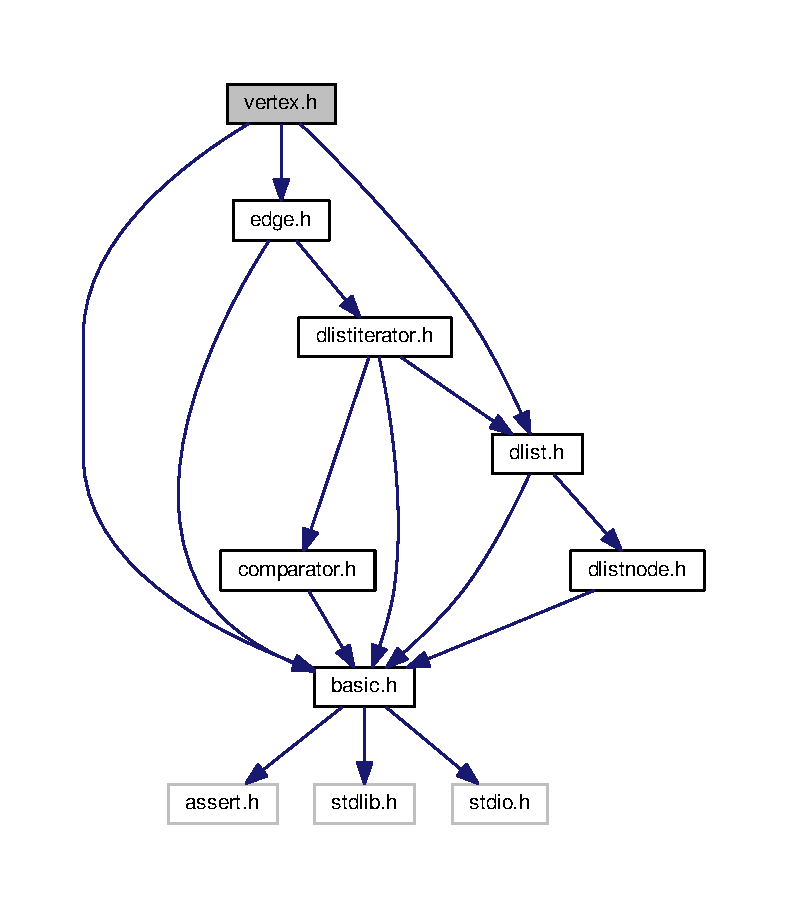
\includegraphics[width=350pt]{vertex_8h__incl}
\end{center}
\end{figure}
This graph shows which files directly or indirectly include this file\+:\nopagebreak
\begin{figure}[H]
\begin{center}
\leavevmode
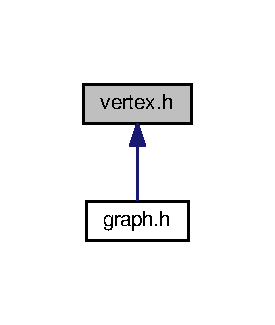
\includegraphics[width=132pt]{vertex_8h__dep__incl}
\end{center}
\end{figure}
\subsection*{Data Structures}
\begin{DoxyCompactItemize}
\item 
struct \hyperlink{structVertex}{Vertex}
\begin{DoxyCompactList}\small\item\em A vertex in a graph is just a container of a doubly linked list of edges. \end{DoxyCompactList}\end{DoxyCompactItemize}
\subsection*{Functions}
\begin{DoxyCompactItemize}
\item 
\hyperlink{structVertex}{Vertex} $\ast$ \hyperlink{vertex_8h_a2b0e1cc520866fea2533679b08ef2232}{vertex\+\_\+new} (void)
\begin{DoxyCompactList}\small\item\em Allocates and initializes a new vertex. \end{DoxyCompactList}\item 
void \hyperlink{vertex_8h_a4b22b5408ae9b8c8b8f406709d2cd322}{vertex\+\_\+destroy} (\hyperlink{structVertex}{Vertex} $\ast$vertex)
\begin{DoxyCompactList}\small\item\em Simply frees the pointer to the vertex. \end{DoxyCompactList}\item 
void \hyperlink{vertex_8h_ac5190248906c628d881fedc69b8a5f12}{vertex\+\_\+destroy\+All} (\hyperlink{structVertex}{Vertex} $\ast$vertex)
\begin{DoxyCompactList}\small\item\em Frees the pointer to the vertex and destroys the complete list of edges. \end{DoxyCompactList}\item 
\hyperlink{structDList}{D\+List} $\ast$ \hyperlink{vertex_8h_aa5b93b2ca706759a4e771fa0b5b06d41}{vertex\+\_\+get\+Edges} (\hyperlink{structVertex}{Vertex} $\ast$vertex)
\item 
int \hyperlink{vertex_8h_adcb3e5d01415ff55fcaa67a00f29389c}{vertex\+\_\+get\+Degree} (\hyperlink{structVertex}{Vertex} $\ast$vertex)
\end{DoxyCompactItemize}


\subsection{Detailed Description}
A vertex in a graph. 

\begin{DoxyAuthor}{Author}
Philipp Badenhoop 
\end{DoxyAuthor}
\begin{DoxyDate}{Date}
6 Jun 2016 
\end{DoxyDate}


\subsection{Function Documentation}
\index{vertex.\+h@{vertex.\+h}!vertex\+\_\+destroy@{vertex\+\_\+destroy}}
\index{vertex\+\_\+destroy@{vertex\+\_\+destroy}!vertex.\+h@{vertex.\+h}}
\subsubsection[{\texorpdfstring{vertex\+\_\+destroy(\+Vertex $\ast$vertex)}{vertex_destroy(Vertex *vertex)}}]{\setlength{\rightskip}{0pt plus 5cm}void vertex\+\_\+destroy (
\begin{DoxyParamCaption}
\item[{{\bf Vertex} $\ast$}]{vertex}
\end{DoxyParamCaption}
)}\hypertarget{vertex_8h_a4b22b5408ae9b8c8b8f406709d2cd322}{}\label{vertex_8h_a4b22b5408ae9b8c8b8f406709d2cd322}


Simply frees the pointer to the vertex. 


\begin{DoxyParams}{Parameters}
{\em vertex} & \\
\hline
\end{DoxyParams}
\begin{DoxyAttention}{Attention}
This does not destroy the list of edges! 
\end{DoxyAttention}
\index{vertex.\+h@{vertex.\+h}!vertex\+\_\+destroy\+All@{vertex\+\_\+destroy\+All}}
\index{vertex\+\_\+destroy\+All@{vertex\+\_\+destroy\+All}!vertex.\+h@{vertex.\+h}}
\subsubsection[{\texorpdfstring{vertex\+\_\+destroy\+All(\+Vertex $\ast$vertex)}{vertex_destroyAll(Vertex *vertex)}}]{\setlength{\rightskip}{0pt plus 5cm}void vertex\+\_\+destroy\+All (
\begin{DoxyParamCaption}
\item[{{\bf Vertex} $\ast$}]{vertex}
\end{DoxyParamCaption}
)}\hypertarget{vertex_8h_ac5190248906c628d881fedc69b8a5f12}{}\label{vertex_8h_ac5190248906c628d881fedc69b8a5f12}


Frees the pointer to the vertex and destroys the complete list of edges. 


\begin{DoxyParams}{Parameters}
{\em vertex} & \\
\hline
\end{DoxyParams}
\index{vertex.\+h@{vertex.\+h}!vertex\+\_\+get\+Degree@{vertex\+\_\+get\+Degree}}
\index{vertex\+\_\+get\+Degree@{vertex\+\_\+get\+Degree}!vertex.\+h@{vertex.\+h}}
\subsubsection[{\texorpdfstring{vertex\+\_\+get\+Degree(\+Vertex $\ast$vertex)}{vertex_getDegree(Vertex *vertex)}}]{\setlength{\rightskip}{0pt plus 5cm}int vertex\+\_\+get\+Degree (
\begin{DoxyParamCaption}
\item[{{\bf Vertex} $\ast$}]{vertex}
\end{DoxyParamCaption}
)}\hypertarget{vertex_8h_adcb3e5d01415ff55fcaa67a00f29389c}{}\label{vertex_8h_adcb3e5d01415ff55fcaa67a00f29389c}

\begin{DoxyParams}{Parameters}
{\em vertex} & \\
\hline
\end{DoxyParams}
\begin{DoxyReturn}{Returns}
Get the number of edges which go out of the vertex. 
\end{DoxyReturn}
\index{vertex.\+h@{vertex.\+h}!vertex\+\_\+get\+Edges@{vertex\+\_\+get\+Edges}}
\index{vertex\+\_\+get\+Edges@{vertex\+\_\+get\+Edges}!vertex.\+h@{vertex.\+h}}
\subsubsection[{\texorpdfstring{vertex\+\_\+get\+Edges(\+Vertex $\ast$vertex)}{vertex_getEdges(Vertex *vertex)}}]{\setlength{\rightskip}{0pt plus 5cm}{\bf D\+List}$\ast$ vertex\+\_\+get\+Edges (
\begin{DoxyParamCaption}
\item[{{\bf Vertex} $\ast$}]{vertex}
\end{DoxyParamCaption}
)}\hypertarget{vertex_8h_aa5b93b2ca706759a4e771fa0b5b06d41}{}\label{vertex_8h_aa5b93b2ca706759a4e771fa0b5b06d41}

\begin{DoxyParams}{Parameters}
{\em vertex} & \\
\hline
\end{DoxyParams}
\begin{DoxyReturn}{Returns}
Get the list of edges. 
\end{DoxyReturn}
\index{vertex.\+h@{vertex.\+h}!vertex\+\_\+new@{vertex\+\_\+new}}
\index{vertex\+\_\+new@{vertex\+\_\+new}!vertex.\+h@{vertex.\+h}}
\subsubsection[{\texorpdfstring{vertex\+\_\+new(void)}{vertex_new(void)}}]{\setlength{\rightskip}{0pt plus 5cm}{\bf Vertex}$\ast$ vertex\+\_\+new (
\begin{DoxyParamCaption}
\item[{void}]{}
\end{DoxyParamCaption}
)}\hypertarget{vertex_8h_a2b0e1cc520866fea2533679b08ef2232}{}\label{vertex_8h_a2b0e1cc520866fea2533679b08ef2232}


Allocates and initializes a new vertex. 

\begin{DoxyReturn}{Returns}
The pointer to the new vertex. 
\end{DoxyReturn}

%--- End generated contents ---

% Index
\backmatter
\newpage
\phantomsection
\clearemptydoublepage
\addcontentsline{toc}{chapter}{Index}
\printindex

\end{document}
